\documentclass[11pt]{article}
%DIF LATEXDIFF DIFFERENCE FILE
%DIF DEL old_red.tex   Sat Oct  3 15:19:31 2026
%DIF ADD new_red.tex   Sat Oct  3 15:19:31 2026
\usepackage[utf8]{inputenc}
\usepackage{amsmath,amssymb}
\usepackage{graphicx}
\usepackage{booktabs}
%DIF 6a6
\usepackage{caption}   % multi-paragraph captions (fig:octet) %DIF > 
%DIF -------
\usepackage{authblk}
\usepackage[margin=1in]{geometry}
\usepackage[hidelinks]{hyperref}

\newcommand{\TODO}[1]{\textbf{[TO MEASURE: #1]}}

\title{A 3D Multiphase Continuum \DIFdelbegin \DIFdel{Computational }\DIFdelend Model for Atoms \DIFaddbegin \DIFadd{and the Periodic Table}\DIFaddend }

\author[1]{Claes Johnson}
\affil[1]{KTH Royal Institute of Technology, Stockholm, Sweden \\
\texttt{claesjohnson@gmail.com}}
\date{\today \\[0.4em]
\small\textit{Mathematical formulation \DIFaddbegin \DIFadd{and the p5.js templates }\DIFaddend by the author;\DIFdelbegin \DIFdel{implementation developed}\DIFdelend } \\
\small\DIFdelbegin \DIFdel{\textit{with AI assistance (Claude, Anthropic).}}\DIFdelend \DIFaddbegin \DIFadd{\textit{developed from them with AI assistance (Claude, Anthropic).}}\DIFaddend }
%DIF PREAMBLE EXTENSION ADDED BY LATEXDIFF
%DIF UNDERLINE PREAMBLE %DIF PREAMBLE
\RequirePackage[normalem]{ulem} %DIF PREAMBLE
\RequirePackage{color}\definecolor{RED}{rgb}{1,0,0}\definecolor{BLUE}{rgb}{0,0,1} %DIF PREAMBLE
\providecommand{\DIFaddtex}[1]{{\protect\color{blue}\uwave{#1}}} %DIF PREAMBLE
\providecommand{\DIFdeltex}[1]{{\protect\color{red}\sout{#1}}} %DIF PREAMBLE
%DIF SAFE PREAMBLE %DIF PREAMBLE
\providecommand{\DIFaddbegin}{} %DIF PREAMBLE
\providecommand{\DIFaddend}{} %DIF PREAMBLE
\providecommand{\DIFdelbegin}{} %DIF PREAMBLE
\providecommand{\DIFdelend}{} %DIF PREAMBLE
\providecommand{\DIFmodbegin}{} %DIF PREAMBLE
\providecommand{\DIFmodend}{} %DIF PREAMBLE
%DIF FLOATSAFE PREAMBLE %DIF PREAMBLE
\providecommand{\DIFaddFL}[1]{\DIFadd{#1}} %DIF PREAMBLE
\providecommand{\DIFdelFL}[1]{\DIFdel{#1}} %DIF PREAMBLE
\providecommand{\DIFaddbeginFL}{} %DIF PREAMBLE
\providecommand{\DIFaddendFL}{} %DIF PREAMBLE
\providecommand{\DIFdelbeginFL}{} %DIF PREAMBLE
\providecommand{\DIFdelendFL}{} %DIF PREAMBLE
%DIF HYPERREF PREAMBLE %DIF PREAMBLE
\providecommand{\DIFadd}[1]{\texorpdfstring{\DIFaddtex{#1}}{#1}} %DIF PREAMBLE
\providecommand{\DIFdel}[1]{\texorpdfstring{\DIFdeltex{#1}}{}} %DIF PREAMBLE
\providecommand{\DIFscaledelfig}{0.5}
%DIF HIGHLIGHTGRAPHICS PREAMBLE %DIF PREAMBLE
\RequirePackage{settobox} %DIF PREAMBLE
\RequirePackage{letltxmacro} %DIF PREAMBLE
\newsavebox{\DIFdelgraphicsbox} %DIF PREAMBLE
\newlength{\DIFdelgraphicswidth} %DIF PREAMBLE
\newlength{\DIFdelgraphicsheight} %DIF PREAMBLE
% store original definition of \includegraphics %DIF PREAMBLE
\LetLtxMacro{\DIFOincludegraphics}{\includegraphics} %DIF PREAMBLE
\providecommand{\DIFaddincludegraphics}[2][]{{\color{blue}\fbox{\DIFOincludegraphics[#1]{#2}}}} %DIF PREAMBLE
\providecommand{\DIFdelincludegraphics}[2][]{% %DIF PREAMBLE
\sbox{\DIFdelgraphicsbox}{\DIFOincludegraphics[#1]{#2}}% %DIF PREAMBLE
\settoboxwidth{\DIFdelgraphicswidth}{\DIFdelgraphicsbox} %DIF PREAMBLE
\settoboxtotalheight{\DIFdelgraphicsheight}{\DIFdelgraphicsbox} %DIF PREAMBLE
\scalebox{\DIFscaledelfig}{% %DIF PREAMBLE
\parbox[b]{\DIFdelgraphicswidth}{\usebox{\DIFdelgraphicsbox}\\[-\baselineskip] \rule{\DIFdelgraphicswidth}{0em}}\llap{\resizebox{\DIFdelgraphicswidth}{\DIFdelgraphicsheight}{% %DIF PREAMBLE
\setlength{\unitlength}{\DIFdelgraphicswidth}% %DIF PREAMBLE
\begin{picture}(1,1)% %DIF PREAMBLE
\thicklines\linethickness{2pt} %DIF PREAMBLE
{\color[rgb]{1,0,0}\put(0,0){\framebox(1,1){}}}% %DIF PREAMBLE
{\color[rgb]{1,0,0}\put(0,0){\line( 1,1){1}}}% %DIF PREAMBLE
{\color[rgb]{1,0,0}\put(0,1){\line(1,-1){1}}}% %DIF PREAMBLE
\end{picture}% %DIF PREAMBLE
}\hspace*{3pt}}} %DIF PREAMBLE
} %DIF PREAMBLE
\LetLtxMacro{\DIFOaddbegin}{\DIFaddbegin} %DIF PREAMBLE
\LetLtxMacro{\DIFOaddend}{\DIFaddend} %DIF PREAMBLE
\LetLtxMacro{\DIFOdelbegin}{\DIFdelbegin} %DIF PREAMBLE
\LetLtxMacro{\DIFOdelend}{\DIFdelend} %DIF PREAMBLE
\DeclareRobustCommand{\DIFaddbegin}{\DIFOaddbegin \let\includegraphics\DIFaddincludegraphics} %DIF PREAMBLE
\DeclareRobustCommand{\DIFaddend}{\DIFOaddend \let\includegraphics\DIFOincludegraphics} %DIF PREAMBLE
\DeclareRobustCommand{\DIFdelbegin}{\DIFOdelbegin \let\includegraphics\DIFdelincludegraphics} %DIF PREAMBLE
\DeclareRobustCommand{\DIFdelend}{\DIFOaddend \let\includegraphics\DIFOincludegraphics} %DIF PREAMBLE
\LetLtxMacro{\DIFOaddbeginFL}{\DIFaddbeginFL} %DIF PREAMBLE
\LetLtxMacro{\DIFOaddendFL}{\DIFaddendFL} %DIF PREAMBLE
\LetLtxMacro{\DIFOdelbeginFL}{\DIFdelbeginFL} %DIF PREAMBLE
\LetLtxMacro{\DIFOdelendFL}{\DIFdelendFL} %DIF PREAMBLE
\DeclareRobustCommand{\DIFaddbeginFL}{\DIFOaddbeginFL \let\includegraphics\DIFaddincludegraphics} %DIF PREAMBLE
\DeclareRobustCommand{\DIFaddendFL}{\DIFOaddendFL \let\includegraphics\DIFOincludegraphics} %DIF PREAMBLE
\DeclareRobustCommand{\DIFdelbeginFL}{\DIFOdelbeginFL \let\includegraphics\DIFdelincludegraphics} %DIF PREAMBLE
\DeclareRobustCommand{\DIFdelendFL}{\DIFOaddendFL \let\includegraphics\DIFOincludegraphics} %DIF PREAMBLE
%DIF AMSMATHULEM PREAMBLE %DIF PREAMBLE
\makeatletter %DIF PREAMBLE
\let\sout@orig\sout %DIF PREAMBLE
\renewcommand{\sout}[1]{\ifmmode\text{\sout@orig{\ensuremath{#1}}}\else\sout@orig{#1}\fi} %DIF PREAMBLE
\makeatother %DIF PREAMBLE
%DIF COLORLISTINGS PREAMBLE %DIF PREAMBLE
\RequirePackage{listings} %DIF PREAMBLE
\RequirePackage{color} %DIF PREAMBLE
\lstdefinelanguage{DIFcode}{ %DIF PREAMBLE
%DIF DIFCODE_UNDERLINE %DIF PREAMBLE
  moredelim=[il][\color{red}\sout]{\%DIF\ <\ }, %DIF PREAMBLE
  moredelim=[il][\color{blue}\uwave]{\%DIF\ >\ } %DIF PREAMBLE
} %DIF PREAMBLE
\lstdefinestyle{DIFverbatimstyle}{ %DIF PREAMBLE
	language=DIFcode, %DIF PREAMBLE
	basicstyle=\ttfamily, %DIF PREAMBLE
	columns=fullflexible, %DIF PREAMBLE
	keepspaces=true %DIF PREAMBLE
} %DIF PREAMBLE
\lstnewenvironment{DIFverbatim}[1][]{\lstset{style=DIFverbatimstyle}}{} %DIF PREAMBLE
\lstnewenvironment{DIFverbatim*}[1][]{\lstset{style=DIFverbatimstyle,showspaces=true}}{} %DIF PREAMBLE
\lstset{extendedchars=\true,inputencoding=utf8}

%DIF END PREAMBLE EXTENSION ADDED BY LATEXDIFF

\begin{document}
\maketitle

\begin{center}
\fbox{\begin{minipage}{0.92\textwidth}\footnotesize
\textbf{Tracked changes.} This document marks the differences between the version reviewed by the
two referees and the present revision, produced with \texttt{latexdiff}. \uwave{Wavy underline}
marks text added in the revision; \sout{strike-through} marks text removed.

The revision is extensive --- the manuscript has grown from 13 pages to 35, and whole sections are
new --- so long passages appear wholly as additions rather than as edits to existing sentences. The
reasons are set out in the response to the referees.

\textbf{Tables.} Every table was rewritten, and change-markup placed inside a \texttt{tabular}
environment does not typeset. Each table is therefore shown here as a single line giving its
caption, marked as added or removed like any other text, and the tables themselves appear in the
manuscript. Six tables in the reviewed version became nine, with none carried over unchanged: the
two heavy-element tables and all ionization-energy tables were withdrawn, and the fourth-row table,
the packing and capacity tables and the convergence table are new.
\end{minipage}}
\end{center}


\begin{abstract}
RealQM \DIFdelbegin \DIFdel{is a general, in-principle parameter-free, low-cost computational method for
quantum mechanics, formulated as three-dimensional continuum mechanics. The electrons
form a sum of one-electron components, each carrying unit charge on a non-overlapping
domain separated by free
(Bernoulli) boundaries, and }\DIFdelend \DIFaddbegin \DIFadd{models atoms as non-overlapping unit electron charge densities, continuous across free
interfaces, interacting by Coulomb potentials without self-repulsion; }\DIFaddend the ground state \DIFdelbegin \DIFdel{minimises the
standard Coulomb energy over both the components and the domain partition. The method is applied here to the periodic table,
computing total energies and first ionization
energies of all atoms in spherical symmetry, with the whole table covered in about a minute on a laptop. Each electron carries its own energy, so the first ionization energy
is read directly as the valence-electron energy, without aseparate ion calculation.Total energies fall within about one to two percent across the table and ionization
energies within ten to twenty percent, with the correct ionization ordering throughout,
including 4s before 3d across the transition series}\DIFdelend \DIFaddbegin \DIFadd{follows by
parabolic relaxation in three space dimensions. The only number supplied is the nuclear charge $Z$,
and nothing is fitted. Neutral atoms are computed all-electron, hydrogen to krypton, to a few
per cent. Two filled packings appear and no third: the antipodal pair, $2$, and the octet, $8=4{+}4$, two
dual tetrahedra. Row capacities are sums of these alone, $2$, $8$, $18=2{+}8{+}8$,
$32=8{+}8{+}8{+}8$; a period ends when its capacity is exhausted, giving the closures
$2,10,18,36,54,86,118$. Each capacity serves two periods. The charge
per unit radius is $Z/2$ in every shell, fixing atomic size near $2$~a}\DIFaddend .\DIFaddbegin \DIFadd{u.\ independently of
$Z$. Capacities are derived at every $Z$, the filling only to carbon and supplied beyond.
}\DIFaddend \end{abstract}

\medskip
\noindent\textbf{Keywords:} atomic structure; real-space methods; multiphase wave
functions; free-boundary problems; \DIFdelbegin \DIFdel{ionization energies; }\DIFdelend \DIFaddbegin \DIFadd{electron packing; Aufbau principle;
electronegativity; }\DIFaddend imaginary-time propagation\DIFdelbegin \DIFdel{;
electron packing}\DIFdelend .

\section{Introduction}\label{sec:intro}

\DIFdelbegin \DIFdel{This paper applies }\DIFdelend \textbf{RealQM} \DIFdelbegin \DIFdel{--- a 3D continuum-mechanical model of the atom in which the $N$ electrons are represented not as a single antisymmetric wave function on $3N$-dimensional configuration space
but as a sum of $N$ one-electron components on
mutually }\DIFdelend \DIFaddbegin \DIFadd{is a model of atoms and molecules in the form of free-boundary multiphase
continuum mechanics in three space dimensions, based on }\DIFaddend non-overlapping \DIFdelbegin \DIFdel{domains of physical three-dimensional space, separated by a free
boundary, both the components and
the partition being unknowns of a single Coulomb-energy
minimisation }\DIFdelend \DIFaddbegin \DIFadd{unit electron charge
densities meeting with continuity at free interfaces and interacting by Coulomb potentials
without self-repulsion and with kernel potentials. The ground
state is computed as the steady state of a }\emph{\DIFadd{parabolic relaxation}}\DIFadd{, or imaginary time
stepping, which decreases the Coulomb energy while maintaining continuity of charge density
across the interfaces, their position being an unknown of the same dynamics. What is reached is the equilibrium accessible from the
state one starts in, so the minimisation is }\emph{\DIFadd{path dependent}} \DIFaddend --- \DIFaddbegin \DIFadd{ordinarily an invisible
distinction, since that equilibrium is the minimum, but the one that decides the shell structure of atoms. The model is parameter-free: its inputs are the
nuclear charge $Z$ --- the atoms being neutral, the electron count is $Z$ as well --- and the energy
minimised is the Coulomb energy alone, with no constant adjusted anywhere. Computational work scales as
$Z$ times the mesh, since each charge density requires one Poisson solve on a grid in three space
dimensions and a neutral atom carries $Z$ of them; the cost is thus linear in $Z$ at fixed
resolution,
which allows the simulation of large molecules and, with successive model reduction, opens to
clusters of molecules; RealQM applied to molecules, to condensed phases and to nuclei is
presented in companion articles~\mbox{%DIFAUXCMD
\cite{Johnson-RealQM}}\hskip0pt\relax %DIFAUXCMD
.
}

\DIFadd{We here take a different route: atoms in their ground configurations, and the periodic table
they compose. The model is taken entire, in its smallest implementation, with nothing fitted and
nothing carried over from the conventional account.
}

\DIFadd{In an atom the densities arrange themselves about the kernel in }\emph{\DIFadd{shells}}\DIFadd{: an inner
region of tightly bound charge, then successive outer layers, each shell holding a definite
number of densities and separated from the next by a free interface. This shell structure ---
how many charges occupy each shell --- is }\DIFaddend \emph{\DIFdelbegin \DIFdel{in spherical symmetry}%DIFDELCMD < \MBLOCKRIGHTBRACE%%%
\DIFdel{, as a detailed test on the }\textbf{\DIFdel{periodic
table}}%DIFAUXCMD
\DIFdel{: }\DIFdelend \DIFaddbegin \DIFadd{not}} \DIFadd{a result of energy minimisation
}\emph{\DIFadd{only}}\DIFadd{. It comes from the packing, electron by electron, as }\DIFaddend the \DIFdelbegin \DIFdel{total atomic energies, electron packing, and ionization energies of the atoms
across all periods, taken from the
outset as its own subject}\DIFdelend \DIFaddbegin \DIFadd{atom is built: a dynamic Aufbau in which
each new charge either continues to fill the outermost shell or, if that shell is complete,
starts the next. A filled shell is shut to it: the charge in a complete shell is a
more rigid arrangement than that of an arriving electron, and resists its inclusion. Given the structure, the
minimisation then settles the interfaces and the energy (Section~\ref{sec:aufbau}).
}

\DIFadd{An atom is spherically symmetric and its shells are concentric}\DIFaddend . The model \DIFdelbegin \DIFdel{and its wider
development }\DIFdelend \DIFaddbegin \DIFadd{therefore admits a
reduction to a single radial dimension, and it is in that form that the table is computed
here. The reduction is a specialisation of the same Coulomb energy, not a second model; but
radial averaging keeps only the number of charges in a shell and discards their angular
arrangement, which is where the packing lives, so it is the three-dimensional form that
decides a packing question (Section~\ref{sec:radialsolver}).
}

\paragraph{Codes.} \DIFadd{We consider here a }\emph{\DIFadd{minimal implementation}} \DIFaddend --- \DIFdelbegin \DIFdel{molecules, bonding, atomization energies, reactions }\DIFdelend \DIFaddbegin \DIFadd{minimal in the code,
not in the model, which is carried in full }\DIFaddend --- \DIFdelbegin \DIFdel{are given in the de Broglie article~\mbox{%DIFAUXCMD
\cite{Johnson-RealQM} }\hskip0pt\relax %DIFAUXCMD
and the accompanying monograph; the present
paper takes the }\emph{\DIFdel{atoms}} %DIFAUXCMD
\DIFdel{themselves as its subject, in periodic-table detail}\DIFdelend \DIFaddbegin \DIFadd{essentially three lines expressing the update of
the charge densities, the update of the potentials and the update of the free boundary,
iterated to a joint steady state (Section~\ref{sec:algorithm}). It is used in two
forms: spherically symmetric in one dimension, some $175$ lines, covering all $Z$; and fully
three-dimensional, some $300$ lines, used at small $Z$ (Section~\ref{sec:code}). The three-dimensional form is the general one, and the one that
extends to molecules. Both are short enough to be read end to end, so the
claim that nothing is fitted can be checked rather than taken on trust}\DIFaddend .

\DIFdelbegin %DIFDELCMD < \paragraph{Context: one method across the whole table.} %%%
\DIFdel{High-accuracy atomic reference data are assembled from a family of specialised
treatments, each chosen to suit the
system at hand: correlated non-relativistic wave-function methods for the light
atoms~\mbox{%DIFAUXCMD
\cite{SzaboOstlund,ClementiRoetti,Chakravorty}}\hskip0pt\relax %DIFAUXCMD
,
relativistic Dirac--Fock for the
heavy ones~\mbox{%DIFAUXCMD
\cite{Desclaux}}\hskip0pt\relax %DIFAUXCMD
, density-functional and real-space approaches for large-scale
work~\mbox{%DIFAUXCMD
\cite{HK64,KS65,Beck2000}}\hskip0pt\relax %DIFAUXCMD
, alongside tabulated experimental values ~\mbox{%DIFAUXCMD
\cite{NIST-ASD}}\hskip0pt\relax %DIFAUXCMD
;
these reach accuracies far beyond the present model. The test reported }\DIFdelend \DIFaddbegin \paragraph{Objective.} \DIFadd{Let RealQM compute a periodic table from the foundational elements of the
Schr\"odinger equation --- charge densities interacting by Coulomb potentials while carrying kinetic
energy, differing from the textbook form only in that the densities do not overlap but meet with
continuity: the }\emph{\DIFadd{neutral
ground states}}\DIFadd{, and for each of them the }\emph{\DIFadd{total energy}}\DIFadd{, the }\emph{\DIFadd{shell structure}}\DIFadd{, and
the }\emph{\DIFadd{Aufbau}} \DIFadd{by which that structure forms. The result is compared
against the reference atomic energies assembled from specialised
treatments~\mbox{%DIFAUXCMD
\cite{SzaboOstlund,ClementiRoetti,Chakravorty,Desclaux,HK64,KS65,Beck2000,NIST-ASD}}\hskip0pt\relax %DIFAUXCMD
,
each suited to its own range. It should be said at once what those references are, since it
bears on how the comparison can be read: a total electronic energy is }\emph{\DIFadd{not}} \DIFadd{an observable,
so they are not measurements but composites --- measured ionisation energies with the
relativistic, QED and nuclear-motion contributions removed by calculation, and, beyond argon,
Hartree--Fock values computed outright. They therefore already contain standard quantum
mechanics, and agreement with them is not a verdict of one theory against nature
(Section~\ref{sec:TEexplicit}). RealQM does not attempt that kind of accuracy in any case, and
the test intended }\DIFaddend here is of a different kind\DIFdelbegin \DIFdel{. A single, in-principle }\DIFdelend \DIFaddbegin \DIFadd{: one }\DIFaddend parameter-free \DIFdelbegin \DIFdel{scheme is }\DIFdelend \DIFaddbegin \DIFadd{model, based on Coulomb
physics, }\DIFaddend applied uniformly to \DIFdelbegin \emph{\DIFdel{every}} %DIFAUXCMD
\DIFdel{atom --- solved the same way for hydrogen and for uranium, with no
per-element adjustment and no fitted functional --- and asked to reproduce the gross electronic }\DIFdelend \DIFaddbegin \DIFadd{every element and asked for the gross }\DIFaddend structure of the whole table
at once \DIFdelbegin \DIFdel{. What a uniform test of this sort can
establish is not competitive accuracy on any one atom but }\emph{\DIFdel{structural correctness
across scope}}%DIFAUXCMD
\DIFdel{: that one Coulomb-energy minimisation recovers the shell filling, }\DIFdelend \DIFaddbegin \DIFadd{--- a structure that does not depend on the reference energies at all. Every atom is
solved all-electron, with the bare nuclear term throughout and no fitted length anywhere. What
the heavier elements require is not a parameter but resolution: }\DIFaddend the \DIFdelbegin \DIFdel{total-energy trend to a few percent, and }\DIFdelend \DIFaddbegin \DIFadd{innermost shell contracts
as $1/Z$, so the mesh is refined where it must be, and nothing else changes. What is computed throughout is the
}\emph{\DIFadd{ground states}}\DIFadd{, which is what a periodic table is about. Ionization and excitation }\DIFaddend --- \DIFdelbegin \DIFdel{the more discriminating outcome }\DIFdelend \DIFaddbegin \DIFadd{and with
them inertness, the property the noble gases are named for }\DIFaddend --- \DIFdelbegin \DIFdel{the
ionization-energy periodicity and ordering, including $4s$ before $3d$ across the transition series. Uniformity across the table , rather than precision on a single atom, is the property put to the test}\DIFdelend \DIFaddbegin \DIFadd{are treated in upcoming work, as are molecules, condensed phases of thousands of atoms, and nuclei, with
larger implementations of the same three updates~\mbox{%DIFAUXCMD
\cite{Johnson-RealQM}}\hskip0pt\relax %DIFAUXCMD
.
}

\paragraph{The table in two numbers.} \DIFadd{It is worth putting the central claim in front of the
reader at once. The model has two filled packings and no third: the }\emph{\DIFadd{antipodal pair}}\DIFadd{, $2$,
and the }\emph{\DIFadd{octet}}\DIFadd{, $8=4{+}4$, two dual tetrahedra. Every closed-shell element in the table is
a whole number of each:
}


\DIFadd{TABLE --- table without caption
}


\noindent \DIFadd{Seven noble gases from two packings, with nothing left over and no third unit
required. A pair is added only twice in the whole table, entering periods 4 and 5, so oganesson
is three pairs and twenty-eight tetrahedra and nothing else.
Sections~\ref{sec:packing} and~\ref{sec:twoeight} establish the two packings and derive the row
capacities from them}\DIFaddend .

\DIFdelbegin %DIFDELCMD < \paragraph{Ionization energy as a per-electron quantity.} %%%
\DIFdel{The feature that makes
atoms a natural target is that, in this multiphase formulation, each electron
satisfies its own one-electron eigenproblem and therefore carries its own energy
$E_i$ }\DIFdelend \DIFaddbegin \DIFadd{Two things this does }\emph{\DIFadd{not}} \DIFadd{say, stated here so the claim is not read wider than it is.
It fixes how many pairs and octets each closed shell contains, not where they sit radially: the
counting cannot distinguish a pair placed innermost from one placed outermost, and that question
is three-dimensional }\DIFaddend (Section~\DIFdelbegin \DIFdel{\ref{sec:model}). The ionization energy is then the energy of the valence electron }\emph{\DIFdel{directly}}%DIFAUXCMD
\DIFdel{, }%DIFDELCMD < \begin{equation}\label{eq:IE-direct}
%DIFDELCMD < \mathrm{IE} \;=\; |E_{\rm valence}|,
%DIFDELCMD < \end{equation}
%DIFDELCMD < %%%
\DIFdel{not a difference $E(\mathrm{A}^+)-E(\mathrm{A})$ of two large total energies.
This
is consequential numerically. An atomic total energy is large (e.g.\ Ne:
$\approx -128.9$ Ha) while an ionization energy is
small ($\mathrm{IE}_1$ of Ne
$\approx 0.79$ Ha); computing the latter as a difference of the former demands the
total energy to absolute accuracy far beyond $1\%$.
}\DIFdelend \DIFaddbegin \DIFadd{\ref{sec:twoeight}). And it is a decomposition of the row
capacities, not a derivation of them --- that each capacity serves two periods is not accounted
for here, and is the principal thing left open.
}

\paragraph{How this stands to the textbook account.} \DIFadd{By the }\emph{\DIFadd{textbook}} \DIFadd{or }\emph{\DIFadd{orbital}}
\DIFadd{account we mean the standard explanation of the periodic table: the one-electron hydrogenic states
$s,p,d,f$, with capacities $2(2\ell{+}1)$, filled in the Madelung order. It should be said at the
outset that this is }\emph{\DIFadd{not}} \DIFadd{the Schr\"odinger equation. }\DIFaddend The \DIFdelbegin \DIFdel{per-electron route avoids
this entirely: the spectator core never enters~\eqref{eq:IE-direct}, so ionization
energies can be accurate even when absolute total energies are only at the
${\sim}1\%$ level. This division }\DIFdelend \DIFaddbegin \DIFadd{$N$-electron Schr\"odinger equation
has no orbitals }\DIFaddend --- \DIFdelbegin \DIFdel{loose total energies, sharp ionization
energies }\DIFdelend \DIFaddbegin \DIFadd{its solutions are functions on $3N$ variables and carry no $s,p,d,f$ labels }\DIFaddend ---
\DIFdelbegin \DIFdel{is }\DIFdelend \DIFaddbegin \DIFadd{and the orbital scheme is an independent-particle approximation laid over it, with the filling
rules laid over that in turn. Nothing in this paper disputes the Schr\"odinger equation. What is
compared here is one account of }\DIFaddend the \DIFdelbegin \DIFdel{organising idea of }\DIFdelend \DIFaddbegin \DIFadd{table's structure against another.
}

\DIFadd{The comparison is worth making carefully, because the two accounts are strong and weak in
different places and it would be easy to overstate either.
}

\DIFadd{What that account does not derive is the }\emph{\DIFadd{order}}\DIFadd{. The Madelung $(n{+}\ell)$ filling rule has no
accepted derivation from the Schr\"odinger equation; Löwdin set the problem out in this journal in
1969~\mbox{%DIFAUXCMD
\cite{Lowdin1969} }\hskip0pt\relax %DIFAUXCMD
and it has been returned to since without being closed~\mbox{%DIFAUXCMD
\cite{AllenKnight2002,Scerri}}\hskip0pt\relax %DIFAUXCMD
.
The $4s$-before-$3d$ ordering in particular has none, and Hund's rules are likewise empirical
regularities rather than consequences. This matters for the present comparison in a specific way:
in the orbital account the }\emph{\DIFadd{doubling}} \DIFadd{--- each capacity serving two periods --- follows from
Madelung, and is therefore exactly as empirical as Madelung is. Neither account derives it.
}

\DIFadd{Nor is the grouping itself settled. The $(n{+}\ell)$ groups close at $2,4,12,20,38,56,88,120$ ---
}\DIFaddend the \DIFdelbegin \DIFdel{paper}\DIFdelend \DIFaddbegin \emph{\DIFadd{alkaline earths}} \DIFadd{--- which is the left-step arrangement; the conventional table's
noble-gas closures require a different placement laid over it, and whether helium belongs above
beryllium or above neon has been argued for a century. The membership of group~3 is still
disputed. So that picture reproduces the table while leaving open both the filling order and,
arguably, which table is being reproduced}\DIFaddend .

\DIFdelbegin %DIFDELCMD < \paragraph{Contributions.} %%%
\DIFdel{(i) A statement of the multiphase 3D atom model and of
the per-electron energy $E_i$ as the computed ionization energy
}\DIFdelend \DIFaddbegin \DIFadd{Against that, the differences here are these. The capacities come from packing rather than from
angular momentum, and $6$, $10$ and $14$ never appear at any row --- the $p$, $d$ and $f$
sub-shells have no counterpart in this model, while the pair survives, though as two charges at
opposite poles rather than as the $\ell=0$ harmonic. The closures come out at the noble gases
directly, with no second placement rule. The order is partly recovered rather than fitted, by a
build-up that is established to carbon. The doubling is not yet derived, but it has a
direction here that it has nowhere else: it is contained in a single ceiling function, and that
function is what relates an areal capacity to a linear radius }\DIFaddend (Section~\DIFdelbegin \DIFdel{\ref{sec:model}); (ii) a two-scale solution architecture pairing a
spherical inner-shell solve with a valence solve in the resulting pseudo-kernel }\DIFdelend \DIFaddbegin \DIFadd{\ref{sec:twoeight}).
Section~\ref{sec:discussion} takes the comparison further.
}

\paragraph{Comparison with textbook quantum mechanics.} \DIFadd{The two rest on the same ingredients
}\DIFaddend --- \DIFdelbegin \DIFdel{spherical for all results here, full 3D~\mbox{%DIFAUXCMD
\cite{Johnson-RealQM} }\hskip0pt\relax %DIFAUXCMD
for the two geometries
that require it (Section~\ref{sec:twoscale}); (iii) the solution algorithm
(Section~\ref{sec:algorithm}); and (iv) validation
across the periodic table }\DIFdelend \DIFaddbegin \DIFadd{kinetic energy and Coulomb interaction, and nothing else }\DIFaddend --- \DIFdelbegin \DIFdel{first and second ionization energies against NIST, and total energies at the ${\sim}1\%$ level }\DIFdelend \DIFaddbegin \DIFadd{and differ in the form taken by
the wave function. Textbook quantum mechanics uses a single global wave function over a
$3N$-dimensional configuration space, and the Schr\"odinger equation for it is }\emph{\DIFadd{linear}}\DIFadd{.
RealQM uses a sum of one-electron wave functions with local, non-overlapping supports in
three-dimensional physical space, the supports themselves being unknowns, which makes it a
}\emph{\DIFadd{nonlinear}} \DIFadd{free-boundary problem. The physics put in is the same; the form of the
description is not, and the difference is worth stating plainly rather than as a verdict.
}

\DIFadd{Density functional theory is the nearer comparison, since it too works in three dimensions. The
difference is that in RealQM the electrons retain their individuality, by occupying separate
regions of space, and in density functional theory they do not, the state being a single common
density.
}

\DIFadd{Exclusion is realised differently in each }\DIFaddend --- \DIFdelbegin \DIFdel{together with the numerical
properties of the solver (Sections~\ref{sec:results}--\ref{sec:convergence}). }\DIFdelend \DIFaddbegin \DIFadd{by
antisymmetry of a function on configuration space, or by non-overlap of domains in
three-space --- and neither is shown here to be an approximation to the other. What is
compared in this paper is what each produces for the periodic table. The reader should take
the wider ontological reading advanced elsewhere~\mbox{%DIFAUXCMD
\cite{Johnson-RealQM} }\hskip0pt\relax %DIFAUXCMD
as speculative,
pending evidence stronger than atomic energetics can supply; nothing here depends on it.
}\DIFaddend 

\section{The multiphase atom model}\label{sec:model}
\DIFdelbegin %DIFDELCMD < 

%DIFDELCMD < %%%
\DIFdel{We summarise }\DIFdelend \DIFaddbegin 

\paragraph{Notation.} \DIFadd{Three symbols recur and are kept distinct throughout. $Z$ is the nuclear
charge, and since only neutral atoms are computed here it is also the number of electrons and so the
number of charge densities. $N$ is the number of points of the uniform radial mesh ($N=400$ through
argon, $N=800$ beyond it). $N_s$ is the occupancy of shell $s$, the number of unit charges smeared
into that shell's density.
}

\DIFadd{RealQM models Coulomb interaction between non-overlapping unit electron charge densities
and point-like kernels, posed as a multiphase free-boundary problem of continuum
mechanics. Each electron is one unit of charge spread as a density
over a domain of three-dimensional space; the domains tile space without overlapping; the
densities meet with continuity on a free boundary, its position determined by the solution
rather than imposed; and the only interaction is the ordinary Coulomb one, between the densities
themselves and between each density and the kernels: the kinetic energy of the densities and
their Coulomb energy are the whole of the functional. We summarise below }\DIFaddend only what is
needed here; derivations are in~\cite{Johnson-RealQM}. For an atom of nuclear charge $Z$ the
$N$-electron wave function \DIFdelbegin \DIFdel{is
}\DIFdelend \DIFaddbegin \DIFadd{$\Psi\in H^1(\mathbb{R}^3)$ has the form
}\DIFaddend \begin{equation}\label{eq:Psi-sum}
\Psi(\mathbf{x}) = \sum_{i=1}^{N} \psi_i(\mathbf{x}),
\qquad \psi_i \in H^1(\Omega_i),
\qquad \int_{\Omega_i} \psi_i^2 \, d\mathbf{x} = 1,
\end{equation}
on a partition of $\mathbb{R}^3$ into non-overlapping domains $\Omega_i$ with free
boundaries $\Gamma_i=\partial\Omega_i$. \DIFaddbegin \DIFadd{Hartree atomic units are used throughout. }\DIFaddend The total
energy is the standard Coulomb functional
\begin{equation}\label{eq:TE}
TE(\Psi)=\underbrace{\tfrac12\sum_i\int_{\Omega_i}|\nabla\psi_i|^2}_{\text{kinetic}}
\;+\;\underbrace{\int_{\mathbb{R}^3} W\,\Psi^2}_{\text{kernel--electron}}
\;+\;\underbrace{\sum_i\int_{\Omega_i}\sum_{j\ne i}V_j\,\psi_i^2}_{\text{electron--electron}},
\end{equation}
with kernel potential $W(\mathbf{x})=-Z/|\mathbf{x}|$ and per-electron Hartree
potentials
$V_j(\mathbf{x})=\tfrac12\int_{\Omega_j}\psi_j^2(\mathbf{y})/|\mathbf{x}-\mathbf{y}|\,d\mathbf{y}$;
self-repulsion is excluded by construction ($j\ne i$ on disjoint domains).
\DIFaddbegin 

\DIFadd{What holds a density against its kernel is then the first term. For a single electron the last
term is empty and~\eqref{eq:TE} reduces to the kinetic energy against the kernel attraction
alone, $-\tfrac12\Delta$ against $-Z/r$: that balance, and nothing else, fixes the size of the
density, and for $Z=1$ it is the hydrogen problem. A functional built instead on one common
density $\rho=\sum_i\psi_i^2$ integrates $\rho$ against itself, so the same balance carries a
repulsion of the electron with its own field and the density comes out too diffuse; removing
that term afterwards is what a self-interaction correction is for. Here there is nothing to
remove.
}

\DIFaddend Stationarity in $\psi_i$ at fixed $\Omega_i$ gives the one-electron eigenproblem
\begin{equation}\label{eq:Hi}
\mathcal{H}_i\psi_i\equiv\Bigl(-\tfrac12\Delta + W + 2\!\sum_{j\ne i}V_j\Bigr)\psi_i = E_i\psi_i
\ \text{ in }\Omega_i,
\qquad \frac{\partial\psi_i}{\partial n}=0 \ \text{ on }\Gamma_i,
\end{equation}
with continuity of $\psi_i$ across the inter-electron interface and the homogeneous
Neumann condition together constituting the \textbf{Bernoulli free-boundary
condition}. Spatial exclusion plays the role of the Pauli principle: the electrons
occupy disjoint territories rather than antisymmetrised orbitals.

\DIFdelbegin %DIFDELCMD < \paragraph{The per-electron energy is the ionization energy.} %%%
\DIFdel{Equation~\eqref{eq:Hi}
gives each electron a well-defined energy $E_i$ }\DIFdelend \DIFaddbegin \DIFadd{For an atom the model reduces to spherical symmetry }\DIFaddend --- \DIFdelbegin \DIFdel{its kinetic energy plus its
attraction to the kernel plus its interaction with the field of the other
electrons. For the valence electron, $|E_{\rm valence}|$ is the energy required to
remove it, i.e.\ the ionization energy~\eqref{eq:IE-direct}. The second ionization
energy is obtained from the valence energy of the singly-ionized atom , recomputed
with the outer electron removed and the remaining partition relaxed. Because the
inner electrons are spectators to this process, the accuracy of $\mathrm{IE}$ is
controlled by the valence solve and not by the (looser) accuracy of the core.
}%DIFDELCMD < 

%DIFDELCMD < \section{Two-scale solution: spherical core, 3D valence}\label{sec:twoscale}
%DIFDELCMD < 

%DIFDELCMD < %%%
\DIFdel{The per-electron structure permits a computation that mirrors the physics: the
spectator core is treated cheaply in spherical symmetry , and only the valence
electrons --- which determine the ionization energies --- are treated explicitly in
3D.
}%DIFDELCMD < 

%DIFDELCMD < \paragraph{Inner shells (spherical).} %%%
\DIFdel{The closed inner shells are solved by a one-dimensional radial reduction of \eqref{eq:Psi-sum}--\eqref{eq:Hi}: radial
densities $u(r)$ with free boundaries between shells set by continuity of $u$. The
converged core supplies an effective }\textbf{\DIFdel{pseudo-kernel}}
%DIFAUXCMD
%DIFDELCMD < \begin{equation}\label{eq:pseudokernel}
%DIFDELCMD < V_{\rm kernel}(r) = -\frac{Z_{\rm kernel}}{r}\ \ (r>r_c),
%DIFDELCMD < \qquad Z_{\rm kernel} = Z - N_{\rm core},
%DIFDELCMD < \end{equation}
%DIFDELCMD < %%%
\DIFdel{smoothly softened for $r\le r_c$, where $Z_{\rm kernel}$ is the nuclear charge
screened by the $N_{\rm core}$ core electrons and the softening radius $r_c$ is read
off the converged core density. Crucially, $r_c$ is thereby }\emph{\DIFdel{determined by the
core solve rather than fitted}}%DIFAUXCMD
\DIFdel{, so the valence calculation carries no per-element
empirical parameter.
}%DIFDELCMD < 

%DIFDELCMD < \paragraph{Valence electrons.} %%%
\DIFdel{In the general two-scale method the valence electrons
are solved explicitly on a 3D grid in the pseudo-kernel~\eqref{eq:pseudokernel},
retaining the angular (sub-shell) structure the radial reduction cannot represent.
}\emph{\DIFdel{In this paper the valence is solved in the same spherical reduction}}
%DIFAUXCMD
\DIFdel{(Section~\ref{sec:radialsolver}); the full 3D solve is reserved for the two geometries
that require it (the closed octet and the interpenetrating $4s/3d$). Either way the
per-electron energies $E_i$ from~\eqref{eq:Hi} give the ionization energies
through~\eqref{eq:IE-direct}, and the loose ${\sim}1\%$ accuracy of the spherical core
enters only through the effective potential it presents to the valence, to which
$\mathrm{IE}$ is far less sensitive than to the core energy itself.
}%DIFDELCMD < 

%DIFDELCMD < \subsection{The spherically-reduced solver}\label{sec:radialsolver}
%DIFDELCMD < 

%DIFDELCMD < %%%
\DIFdel{Every result in this paper is computed with the spherical (1D radial) reduction of the
model, which we state explicitly. The atom has shells$s=0,\dots,S{-}1$; shell $s$
carries $N_s$ electrons as a radial amplitude $u_s(r)$ on $[R_{s-1},R_s]$ (with
$R_{-1}=0$, $R_{S-1}=\infty$). With the $s$-wave radial Laplacian
$\Delta u = u'' + \tfrac{2}{r}u'$ and Hartree atomic units, }\DIFdelend \DIFaddbegin \DIFadd{a specialisation available because
atoms are spherical --- with $\Psi$ a function of $r$ alone, the domains $\Omega_i$ concentric
shells, }\DIFaddend the \DIFdelbegin \DIFdel{per-electron operator,
its imaginary-time relaxation to the ground state, and the per-electron Hartree
potential of the }\emph{\DIFdel{other}} %DIFAUXCMD
\DIFdel{shells are
}%DIFDELCMD < \begin{align}
%DIFDELCMD < H_s &= -\tfrac12\Delta - \frac{Z}{r} + W_s(r), &
%DIFDELCMD < \frac{\partial u_s}{\partial\tau} &= -H_s u_s, \label{eq:radial-itp}\\
%DIFDELCMD < -\Delta W_s &= 4\pi\!\!\sum_{t\neq s}\! |u_t|^2, &
%DIFDELCMD < &W_s(r)=\tfrac1r\!\int_0^r\!\!\rho_{\neq s}4\pi r'^2dr' + \!\int_r^\infty\!\!\rho_{\neq s}4\pi r'dr', \label{eq:radial-hartree}
%DIFDELCMD < \end{align}
%DIFDELCMD < %%%
\DIFdelend \DIFaddbegin \DIFadd{free interfaces $\Gamma_i$ radii $R_s$, and }\DIFaddend the same-shell self-term \DIFaddbegin \DIFadd{of a shell
holding $N_s$ charges }\DIFaddend reduced by $(N_s{-}1)/N_s$ \DIFdelbegin \DIFdel{. The interfaces $R_s$ are free
(Bernoulli)boundaries, fixed by continuity of the amplitude, and each shell is
normalised:
}%DIFDELCMD < \begin{equation}\label{eq:radial-bc}
%DIFDELCMD < u_s(R_s)=u_{s+1}(R_s), \qquad 4\pi\!\int_0^\infty |u_s|^2 r^2\,dr = N_s .
%DIFDELCMD < \end{equation}
%DIFDELCMD < %%%
\DIFdel{The total energy (half-Hartree, no double counting) and the per-electron eigenvalue
(full Hartree) --- the latter the ionization energy }\DIFdelend \DIFaddbegin \DIFadd{(Section~\ref{sec:radialsolver}); the reduced
equations are exhibited by the code }\DIFaddend of Section~\DIFdelbegin \DIFdel{\ref{sec:model} --- are
}%DIFDELCMD < \begin{equation}\label{eq:radial-E}
%DIFDELCMD < E=\sum_s 4\pi\!\int\!\Big[\tfrac12|u_s'|^2-\tfrac{Z}{r}|u_s|^2+\tfrac12 W_s|u_s|^2\Big]r^2dr,
%DIFDELCMD < \qquad \varepsilon_s=\frac{\langle u_s|H_s|u_s\rangle}{N_s},\ \ \mathrm{IE}=|\varepsilon_{\rm valence}|.
%DIFDELCMD < \end{equation}
%DIFDELCMD < %%%
\DIFdel{The scheme is
discretised on a uniform grid $r_i=ih$ with an explicit step
$\Delta\tau=\tfrac12 h^2$ (first order, cusp-limited; Section~\ref{sec:convergence}).
For $Z>18$ }\DIFdelend \DIFaddbegin \DIFadd{\ref{sec:code}. Every atom reported here is
solved all-electron, }\DIFaddend the nuclear term \DIFdelbegin \DIFdel{is replaced by the pseudo-kernel
$Z/r\to Z_{\rm ker}/\max(r,r_c)$ of~\eqref{eq:pseudokernel} with a Neumann inner
boundary $u'(r_c)=0$, confining the valence outside the core }\DIFdelend \DIFaddbegin \DIFadd{the bare $-Z/r$ throughout, with no core radius, no
screened kernel and no fitted length anywhere}\DIFaddend .

\DIFaddbegin \begin{figure}[t]
\centering
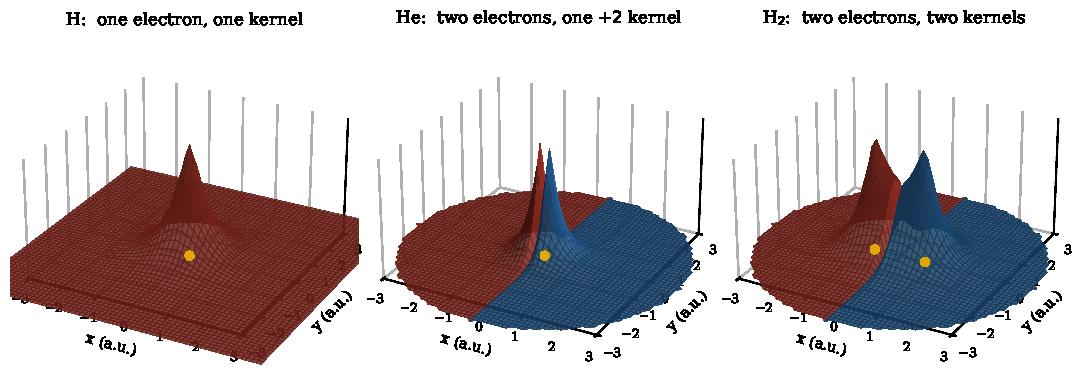
\includegraphics[width=\textwidth]{fig_essence.pdf}
\caption{\DIFaddFL{The model in three dimensions: charge density as surface elevation over the plane
through the kernels, one colour per electron domain, kernels marked in yellow on the base
plane. }\textbf{\DIFaddFL{H}}\DIFaddFL{: a single domain. }\textbf{\DIFaddFL{He}}\DIFaddFL{: two one-electron domains on one $+2$ kernel,
meeting at a free interface through the nucleus. }\textbf{\DIFaddFL{H$_2$}}\DIFaddFL{: the same two domains with the
kernels drawn apart to the bond length. He and H$_2$ differ only in where the kernels sit,
which is this model's account of what a bond is. The quantity drawn is $|\psi_i|^2$ on the
territory domain $i$ holds, unowned cells left unpainted, so the interface appears as the ridge
between the two surfaces rather than as overlapping clouds. Cartesian grid, $120^3$ over a box
of $8$~a.u., $\varepsilon=h$. The figure is of the }\emph{\DIFaddFL{partition}} \DIFaddFL{and no energy is quoted from it:
these are three-dimensional runs, whereas the energies of Table~\ref{tab:TE} come from the
spherically homogenised solver, and neither H nor H$_2$ appears there at all.}}
\label{fig:essence}
\end{figure}

\DIFaddend \section{Algorithm: the three-line solver}\label{sec:algorithm}

The \DIFdelbegin \DIFdel{radial system of Section~\ref{sec:radialsolver} }\DIFdelend \DIFaddbegin \DIFadd{system }\DIFaddend is solved by three coupled relaxations to a joint steady state --- the
\emph{three-line solver}. \DIFdelbegin \DIFdel{At each time }\DIFdelend \DIFaddbegin \DIFadd{We state them for the general case of
Section~\ref{sec:model}; the spherical homogenisation stated there is the
special case in which the domains are concentric shells and each $\psi_i$ depends on $r$ alone.
At each }\DIFaddend step, for every \DIFdelbegin \DIFdel{shell $s$}\DIFdelend \DIFaddbegin \DIFadd{domain $\Omega_i$}\DIFaddend :
\begin{enumerate}\setlength{\itemsep}{1pt}
\item \textbf{\DIFdelbegin \DIFdel{Imaginary-time propagation}\DIFdelend \DIFaddbegin \DIFadd{Imaginary time stepping}\DIFaddend } of the amplitude \DIFdelbegin \DIFdel{,
$\partial_\tau u_s=-H_s u_s$~\eqref{eq:radial-itp}, relaxing
$u_s$ }\DIFdelend \DIFaddbegin \DIFadd{--- parabolic relaxation ---
$\partial_\tau \psi_i=-\mathcal{H}_i \psi_i$ with $\mathcal{H}_i$ from~\eqref{eq:Hi}, relaxing
$\psi_i$ }\DIFaddend toward the lowest eigenfunction of \DIFdelbegin \DIFdel{$H_s$; }\DIFdelend \DIFaddbegin \DIFadd{$\mathcal{H}_i$; $\tau$ is an artificial time
carrying the relaxation and has no physical meaning, only the steady state being used;
}\DIFaddend \item a \textbf{Poisson \DIFdelbegin \DIFdel{/ shell-theorem }\DIFdelend solve} for the per-electron \DIFdelbegin \DIFdel{Hartree potential $W_s$~\eqref{eq:radial-hartree}}\DIFdelend \DIFaddbegin \DIFadd{potential $V_i$, which in spherical
symmetry is the shell-theorem integral over the other shells}\DIFaddend ;
\item a \textbf{boundary move}: each \DIFdelbegin \DIFdel{shell radius $R_s$ }\DIFdelend \DIFaddbegin \DIFadd{interface $\Gamma_i$ }\DIFaddend is shifted in the direction that
\emph{decreases the jump} of \DIFdelbegin \DIFdel{$u$ }\DIFdelend \DIFaddbegin \DIFadd{$\Psi$ }\DIFaddend across it, driving \DIFdelbegin \DIFdel{the interface }\DIFdelend \DIFaddbegin \DIFadd{it }\DIFaddend toward the continuity \DIFdelbegin \DIFdel{~\eqref{eq:radial-bc} }\DIFdelend \DIFaddbegin \DIFadd{that
$\Psi\in H^1$ demands }\DIFaddend --- the Bernoulli free-boundary condition.
\end{enumerate}
After each step \DIFdelbegin \DIFdel{$u_s$ is renormalised~\eqref{eq:radial-bc}}\DIFdelend \DIFaddbegin \DIFadd{$\psi_i$ is renormalised}\DIFaddend ; at convergence the boundaries are stationary and the
per-electron energy is the Rayleigh quotient\DIFdelbegin \DIFdel{$\varepsilon_s$~\eqref{eq:radial-E}}\DIFdelend , supplying the \DIFdelbegin \DIFdel{ionization energy
through~\eqref{eq:IE-direct}.
Each }\DIFdelend \DIFaddbegin \DIFadd{per-shell energies.
In the spherical case the scheme is discretised on a uniform grid $r_i=ih$ with an explicit
step $\Delta\tau=\tfrac12 h^2$ (first order, cusp-limited; Section~\ref{sec:convergence}), and
each }\DIFaddend of the three is a single one-dimensional grid sweep on $r_i=ih$, so every atom converges in a fraction of a second and the whole periodic table
in about a minute on a laptop.

\DIFdelbegin %DIFDELCMD < \section{Results: total energies, packing, and ionization across the periodic table}%%%
\DIFdelend \DIFaddbegin \paragraph{The algorithm is a relaxation, not a global minimisation.} \DIFadd{This is worth stating
at the outset because it governs how the results below should be read. None of the three
updates searches the space of configurations; each is a parabolic relaxation --- the
amplitude down the gradient of $H_s$, the potential toward its Poisson source, the interface
toward continuity --- and what they reach together is a }\emph{\DIFadd{steady state}}\DIFadd{, a configuration
at which all three forces balance. Such a state is a critical point of the Coulomb functional,
and the ground state is one; but the relaxation arrives at whichever equilibrium lies at the
end of the path it is on, and there is no step at which a lower configuration elsewhere in the
space is offered and refused. Energy minimisation here is therefore }\emph{\DIFadd{path dependent}}\DIFadd{:
what is computed is the equilibrium reachable from the initial state, not the infimum over all
states.
}

\DIFadd{Ordinarily this distinction is invisible, because the reachable equilibrium }\emph{\DIFadd{is}} \DIFadd{the
minimum. It becomes the whole point in Section~\ref{sec:aufbau}, where a lower configuration
exists, is never reached, and is not the physical one either --- so that the path, and not the
infimum, is what selects the structure of the atom.
}

\section{What the spherical homogenisation costs}\label{sec:radialsolver}

\paragraph{What the $(N_s{-}1)/N_s$ factor is, and what the homogenisation costs.}
\DIFadd{The factor is not a correction added to the model: it is forced by the homogenisation --- by
replacing the $N_s$ discrete charges of a shell with their spherical average, which is what
makes the problem radial and hence one-dimensional. In
3D the $N_s$ electrons of a shell occupy $N_s$ separate one-electron domains and the
$i\neq j$ rule counts $N_s(N_s{-}1)/2$ pairs. Smearing them into one spherical density
of charge $N_s$ makes the Hartree self-energy count $N_s^2$ pairs, of which $N_s$ are
spurious self-pairs; multiplying by $(N_s{-}1)/N_s$ removes exactly those. Nothing is
fitted, and the parameter-free character of the model is untouched.
}

\DIFadd{Smearing does a second thing, however, and this one is a genuine loss. It replaces the
actual pair }\emph{\DIFadd{separations}} \DIFadd{by their spherical average. The charges of a shell sit
as far apart as the shell allows --- antipodal for $N_s=2$, trigonal for $3$,
tetrahedral for $4$ --- and those arrangements repel less than the angular average. For
unit charges at a common radius $R$ (units of $1/R$):
}


\DIFadd{TABLE --- table without caption
}


\DIFadd{So the homogenised shell has the pair }\emph{\DIFadd{count}} \DIFadd{right and the pair
}\emph{\DIFadd{geometry}} \DIFadd{wrong, overestimating intra-shell repulsion by a factor $1.6$--$2$. Most
of that is absorbed by the shell radius, which is free and expands until the energy
re-minimises; what survives appears as a systematic under-binding, and it is largest at
$N_s=2$, where the ratio is largest. Helium is the clean test --- one shell, two
electrons, no core, no $r_c$, and a reference that is exactly known as a nonrelativistic
eigenvalue rather than inferred from measurement --- and it under-binds by $2.0\%$
(Table~\ref{tab:TE}), with the sign the table predicts.
}

\DIFadd{The thing discarded is precisely the angular correlation, which is what packing
}\emph{\DIFadd{means}}\DIFadd{. This is why the homogenised model cannot adjudicate a packing question on
energetic grounds --- it has no angles with which to tell $4{+}4$ from a single
$8$-shell --- and why the capacities of Section~\ref{sec:packing} are established by the
counting argument and the 3D solve rather than by the radial energies.
}

\section{Results: total energies, packing, and electronegativity}\DIFaddend \label{sec:results}

We report three results. The electron packing (Section~\ref{sec:packing}) and the
all-electron total energies \DIFdelbegin \DIFdel{of the first three periods (Section~\ref{sec:TEexplicit} }\DIFdelend \DIFaddbegin \DIFadd{(Sections~\ref{sec:TEexplicit} and~\ref{sec:TE4}}\DIFaddend )
come from the \DIFdelbegin \DIFdel{spherically-reduced }\DIFdelend \DIFaddbegin \DIFadd{spherically-homogenised }\DIFaddend (1D radial) solver applied to every electron\DIFdelbegin \DIFdel{. The
full main-group periodic table }\DIFdelend \DIFaddbegin \DIFadd{, with the
bare nuclear charge and no fitted length. The electronegativities
}\DIFaddend (Section~\DIFdelbegin \DIFdel{\ref{sec:frozencore}) is then reached by the
two-scale frozen-core decomposition of Section~\ref{sec:twoscale}: an inner core taken
from reference data~\mbox{%DIFAUXCMD
\cite{ClementiRoetti,Desclaux} }\hskip0pt\relax %DIFAUXCMD
plus the RealQM valence computed in
its pseudo-kernel. The transition and inner-transition elements (the $d$- and $f$-blocks) enter only as closed
buried cores }\DIFdelend \DIFaddbegin \DIFadd{\ref{sec:chi}) follow from the same shell energies. The energies cover periods~1--4, hydrogen to
krypton, $Z=1$--$36$, with nothing adjusted anywhere: the only quantity that varies across the range
is the mesh, chosen by $Z$ so that the innermost shell stays resolved }\DIFaddend --- \DIFdelbegin \DIFdel{physically appropriate, since their electrons lie }\emph{\DIFdel{inside}} %DIFAUXCMD
\DIFdel{the valence and barely participate in chemistry }\DIFdelend \DIFaddbegin \DIFadd{$N=400$ through argon,
$N=800$ from potassium }\DIFaddend --- \DIFdelbegin \DIFdel{and are not resolved individually;
``main group'' below means groups 1--2 and 13--18. Ionization energies
}\DIFdelend \DIFaddbegin \DIFadd{which is a discretisation and not a parameter of the model. What is bounded at argon is not the calculation but the
}\emph{\DIFadd{build-up}}\DIFadd{: from scandium the next charge belongs inside a shell already occupied, which an
outward build-up cannot do, so the fourth row's configurations are supplied rather than derived
}\DIFaddend (Section~\DIFdelbegin \DIFdel{\ref{sec:ie})are summarised last}\DIFdelend \DIFaddbegin \DIFadd{\ref{sec:dblock})}\DIFaddend .

\subsection{Electron packing: 4+4, not 8}\label{sec:packing}

\DIFdelbegin \DIFdel{For each atom the shell packing is determined by total energy}\DIFdelend \DIFaddbegin \DIFadd{The shell packing of each atom is supplied by the build-up of
Section~\ref{sec:aufbau}, not chosen by fitting energies}\DIFaddend . Two findings are
robust across $Z=2$--$18$. \emph{First}, comparing shells of capacity 2, 4, 6, 8,
the \textbf{cap-4} packing matches reference total energies best everywhere: a
capacity-8 shell over-binds by $+9\%$ to $+22\%$ (worsening with $Z$), and a closed
octet is realised only as \textbf{4+4}, never as a single 8-shell --- the
geometrically expected result, since four unit charges pack as a stable tetrahedron
while eight on one shell do not. \DIFaddbegin \DIFadd{Here }\textbf{\DIFadd{4+4}} \DIFadd{means two }\emph{\DIFadd{radial}} \DIFadd{shells of four,
which is all a spherically homogenised model can mean by it; whether the two tetrahedra close onto
a common sphere is a separate, three-dimensional question, taken up in
Section~\ref{sec:twoeight}. }\DIFaddend \emph{Second}, distributing each period's electrons
\emph{evenly} across its cap-4 shells (balanced filling) rather than greedily
reproduces the classic configurations 2+2+1 (B), 2+2+2 (C), 2+3+2 (N), 2+3+3 (O) and
tightens the energies (e.g.\ C: $+4.4\%$ greedy $\to -1.1\%$ balanced).

The organising principle is geometric: each electron is a localised cloud whose
\emph{size} is set by its distance from the kernel --- inner electrons compact, outer
ones diffuse --- and the shells are the close-packings (capacities $2$ and $4$) of these
clouds. Different packings of the same atom have different energies, and ---
importantly --- the \emph{unconstrained} energy minimum is \emph{not} the physical
configuration: in the 1D solver it favours the over-packed capacity-8 shell, the radial
model lacking the angular exclusion that makes 8-on-a-shell unstable (a first signal
that the closed shell is intrinsically three-dimensional). The physical packing is fixed
instead by the build-up (Aufbau) of the atom, electron by electron\DIFdelbegin \DIFdel{. In this paper we
therefore take the packing as the classic cap-4 configurations, selected by best fit to
the total energies, and defer a }\emph{\DIFdel{dynamical}} %DIFAUXCMD
\DIFdel{Aufbau }\DIFdelend \DIFaddbegin \DIFadd{, which is the subject of
Section~\ref{sec:aufbau}: the constraint that the inner shells are already filled removes
the over-packed arrangements from the search, and among what remains the energy selects
correctly. The capacities themselves are not fitted either }\DIFaddend --- \DIFdelbegin \DIFdel{one that would select the physical packing intrinsically --- to later work; RealQM's task here is to compute the energies of the chosen packings accurately. }\DIFdelend \DIFaddbegin \DIFadd{$2$ and $4{+}4$ are the
$n=1$ and $n=2$ cases of the counting argument of Section~\ref{sec:twoeight}.
}\DIFaddend 


\DIFdelbegin %DIFDELCMD < \subsection{All-electron total energies, periods 1--3}\label{sec:TEexplicit}
%DIFDELCMD < %%%
\DIFdelend \DIFaddbegin \begin{figure}[t]
\centering
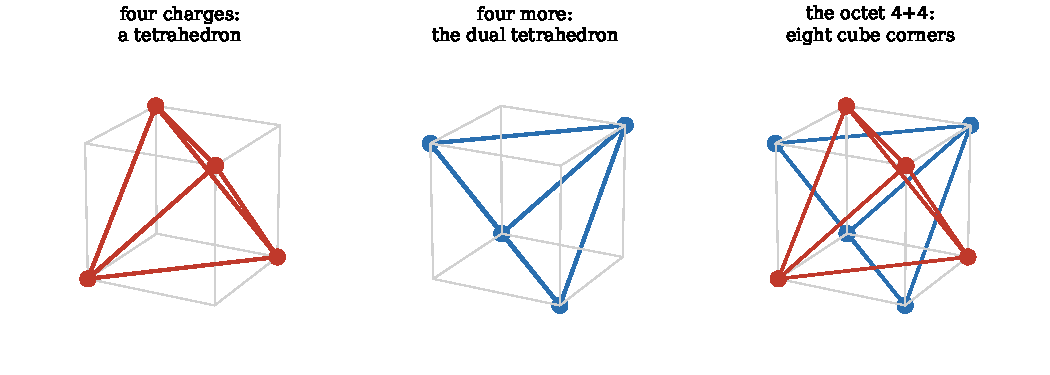
\includegraphics[width=\textwidth]{fig_octet.pdf}
\caption[The octet as $4{+}4$]{\DIFaddFL{The octet as $4{+}4$. Four unit charges on a shell settle as a tetrahedron, the
arrangement that puts them as far apart as a sphere allows. A second four cannot join them ---
the tetrahedron is closed --- but they can occupy the }\emph{\DIFaddFL{dual}} \DIFaddFL{tetrahedron, and the eight
together are the corners of a cube. The two interleave rather than stack: on a cube of side $2$
the charges within one tetrahedron are $2.83$ apart while the nearest charge of the other is at
$2.00$, so every charge's neighbours belong to the opposite four. This is why the closed octet
is $4{+}4$ and never a single shell of eight, which over-binds by $9$--$22\%$
(Section~\ref{sec:packing}); and it is the $n=2$ case of the counting of
Section~\ref{sec:twoeight}, the $n=1$ case being the antipodal pair.
}

\DIFaddFL{The orbital picture makes the same eight as $2{+}6$, an $s$ pair and three $p$ lobes. The two
accounts agree on the number and differ in the decomposition, and it is the decomposition that
bonding geometry sees: $sp^3$ hybridisation exists to turn $2{+}6$ back into four tetrahedral
directions, which $4{+}4$ supplies at the outset.
}

\DIFaddFL{This is Linnett's double quartet~\mbox{%DIFAUXCMD
\cite{Linnett1961}}\hskip0pt\relax %DIFAUXCMD
, which reads Lewis's cubical octet as two
interpenetrating tetrahedral sets of four. Linnett separates the two by }\emph{\DIFaddFL{spin}} \DIFaddFL{--- Fermi
correlation within a quartet, Coulomb correlation between them. The present model contains no
spin, and obtains the same arrangement from Coulomb repulsion and non-overlap alone; what is
offered here is therefore not the decomposition but a derivation of it that does not need spin.
}

\DIFaddFL{The cube drawn here is a }\emph{\DIFaddFL{geometric}} \DIFaddFL{argument and is not what the calculations of this
paper compute. The spherically homogenised solver has no angular coordinate, so its $4{+}4$ is two
nested radial shells; measured, the two tetrahedra come out well separated rather than on a
common sphere (Section~\ref{sec:twoeight}). The cube is what we expect the three-dimensional
form to give, not a result reported here.
}

\DIFaddFL{One classical result must be conceded, and it bounds the claim usefully. For }\emph{\DIFaddFL{four}} \DIFaddFL{points on
a sphere the Coulomb minimum is the regular tetrahedron ($3.6742$ against $3.8284$ for a square),
so the tetrahedron is on firm ground. For }\emph{\DIFaddFL{eight}} \DIFaddFL{on }\emph{\DIFaddFL{one}} \DIFaddFL{sphere it is not the cube but
the square antiprism, by $0.33\%$ ($19.6753$ against $19.7408$), and this is a
theorem~\mbox{%DIFAUXCMD
\cite{Thomson8}}\hskip0pt\relax %DIFAUXCMD
. Two things follow. The antiprism is itself a $4{+}4$ --- two squares
twisted by $45^\circ$ --- so what the theorem refutes is the two-}\emph{\DIFaddFL{tetrahedra}} \DIFaddFL{reading of a
}\emph{\DIFaddFL{single}} \DIFaddFL{sphere, not the $4{+}4$ decomposition. And this model does not place eight charges on
one sphere: a single 8-shell over-binds by $9$--$22\%$ (Section~\ref{sec:packing}) and the octet
is realised over two radii, which a single-sphere theorem does not reach. It does mean the cube
must not be offered as a Coulomb minimum, and we do not offer it as one.}}
\label{fig:octet}
\end{figure}
\DIFaddend 

\DIFaddbegin \subsection{Aufbau: how the shell structure forms}\label{sec:aufbau}

\DIFadd{The shell structure of an atom is not a static fact to be looked up but something that
}\emph{\DIFadd{forms}}\DIFadd{, electron by electron, as the atom is built. Why the structure cannot instead be
obtained by minimising over packings is worth stating precisely, because it turns out to be a
structural property of the model rather than a weakness of the search.
}

\paragraph{The energy is monotone in the packing.} \DIFadd{Comparing candidate packings of the
same atom, the energy decreases without interior minimum as the electrons are gathered
into fewer, more compact shells. The unconstrained minimum is therefore always the most
compact arrangement, in which the core is absorbed into the valence, and it is far from
the reference value:
}



\DIFadd{TABLE --- table without caption
}



\noindent \DIFadd{These energies are computed at $20\,000$ steps on the solver's default mesh, so they differ
in the third decimal from }\DIFaddend Table~\ref{tab:TE}\DIFdelbegin \DIFdel{reports total energies with the balanced cap-4 packing against
near-exact nonrelativistic reference values~\mbox{%DIFAUXCMD
\cite{Chakravorty}}\hskip0pt\relax %DIFAUXCMD
.
}%DIFDELCMD < 

%DIFDELCMD < %%%
\DIFdel{TABLE }\DIFdelend \DIFaddbegin \DIFadd{, which uses the finer settings of the periodic-table scan
}\DIFaddend --- \DIFdelbegin \DIFdel{Total atomic energies (balanced cap-4 packing, spherically-reduced solver) versus near-exact nonrelativistic r
}\DIFdelend \DIFaddbegin \DIFadd{lithium appears here as $-7.547$ and there as $-7.522$. Neither is wrong: each table makes an
internal comparison, one between candidate packings of the same atom and the other between atoms, and
the settings are held fixed within each. They should not be read across.
}\DIFaddend 

The \DIFdelbegin \DIFdel{mean relative error is$1.7\%$ and the maximum $4.6\%$ (Si, S); most atoms fall
within $2.5\%$.
This is comparable to Hartree--Fock accuracy on total energy }\DIFdelend \DIFaddbegin \DIFadd{physical configuration is, in each case, the }\emph{\DIFadd{least}} \DIFadd{bound of the
candidates and simultaneously the closest to the reference. A variational search over
packings is thus not merely unhelpful here; it is anti-correlated with the answer.
}

\paragraph{What a build-up supplies.} \DIFadd{The failure is specific: it occurs only where the
search is free to dissolve an already-formed core. An Aufbau construction never offers
that. Electrons are added one at a time; the parent configuration is inherited; and a
filled packing admits no more. Imposing only those three conditions }\DIFaddend --- \DIFdelbegin \DIFdel{with
the opposite sign of error (RealQM over-binds the heavier atoms of the third period,
where HF
under-binds through missing correlation) }\DIFdelend \DIFaddbegin \DIFadd{and letting the
energy choose among what remains }\DIFaddend --- \DIFdelbegin \DIFdel{obtained from a 1D radial solve with no
basis sets, no antisymmetry, and no two-electron integrals}\DIFdelend \DIFaddbegin \DIFadd{recovers the physical configuration of Li, Be, B and
C with no empirical input, the energy merely breaking ties. Nothing is frozen
numerically: every candidate is solved with all shells, radii and amplitudes relaxed.
}

\DIFadd{This is where the path dependence of Section~\ref{sec:algorithm} becomes the physics rather
than a caveat. The three conditions are not restrictions imposed on a search; they are a
description of the }\emph{\DIFadd{path}} \DIFadd{the atom takes as it forms. An electron arriving at an atom
whose inner shells are already occupied cannot reach them --- not because a rule forbids it,
but because a filled shell is the more rigid of the two. What decides is }\emph{\DIFadd{relative}}
\DIFadd{rigidity, and nothing else could: the interface moves only where one domain's amplitude locally
exceeds the other's, so the comparison is between the two charges and not a property of either
alone. The compact charge of a complete shell wins against the diffuse charge arriving at it;
the newcomer is turned aside and takes the room outside instead. Figure~\ref{fig:lisnaps}
shows this happening --- the core unchanged and centred while the arriving charge is deflected
around it. The merged configuration remains a legitimate
state of lower energy; it is simply not reachable from where the arriving charge starts. The
build-up is thus not a constraint added to repair the minimisation. It }\emph{\DIFadd{is}} \DIFadd{the
minimisation, carried out along the path the atom actually takes, and the physical
configuration is the equilibrium at the end of it}\DIFaddend .

\DIFdelbegin %DIFDELCMD < \subsection{Frozen-core total energies: the floor and the variation}\label{sec:frozencore}
%DIFDELCMD < %%%
\DIFdelend \DIFaddbegin \begin{figure}[t]
\centering
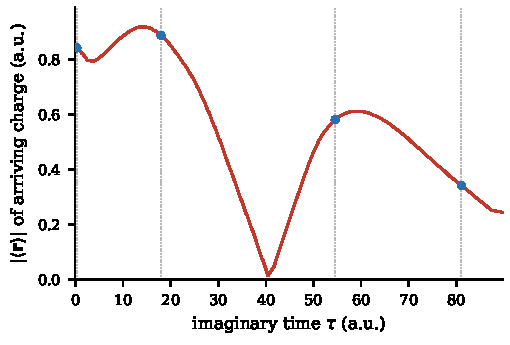
\includegraphics[width=0.62\textwidth]{fig_li_wrap.pdf}
\caption{\DIFaddFL{The build-up as a dynamics: Li$^+$ with one electron added. The arriving charge is
launched as a }\emph{\DIFaddFL{half-shell}} \DIFaddFL{outside the core --- its density concentrated on one side, so
that no shell is present at $\tau=0$ --- and the interface between the two is free thereafter.
Plotted is the distance of the arriving charge's centroid from the kernel against imaginary
time. It falls from $0.84$ to $0.014$ --- essentially through the centre --- then swings back
out: a damped oscillation about the closed shell rather than a decay onto it. The charge wraps
}\emph{\DIFaddFL{around}} \DIFaddFL{the core rather than merging into it. Dotted lines mark the four times shown in
Figure~\ref{fig:lisnaps}. A longer run of the same case carries the oscillation through a
second pass and down to $4.5\%$ of the launch value; the run plotted here stops partway through
the second swing, which is why it ends at $0.24$ rather than near zero. A single $3$-shell lies $1.055$~Ha below $2{+}1$, but that
figure comes from a separate calculation of a }\emph{\DIFaddFL{different configuration}} \DIFaddFL{and the present run
cannot reach it: the solver renormalises each domain to its own occupancy at every step, so the
two charges of the core and the one arriving are fixed by construction and no interface motion can
turn $2{+}1$ into $3$. We therefore do not claim that the relaxation declines an available lower
state. What this run shows is narrower and is what the figures are offered for: }\emph{\DIFaddFL{given}} \DIFaddFL{the
$2{+}1$ occupancies, the arriving charge closes a shell outside the core instead of entering it,
and the core is not invaded. Which of $2{+}1$ and $3$ an atom adopts is a question about
configuration selection, treated in Section~\ref{sec:aufbau}, not one this run answers. All-electron, no
$r_c$, $200^3$; the core is under-bound at this resolution, so no energy or radius is quoted
from the run and none is needed for the statement made.}}
\label{fig:liwrap}
\end{figure}
\DIFaddend 

\DIFdelbegin \DIFdel{A total energy is meaningful only relative to a
reference level. The
absolute number is dominated by the deep inner shells and conveys little on
its own; chemistry and periodicity live in the }\emph{\DIFdel{changes}} %DIFAUXCMD
\DIFdel{of energy across groups and down periods. The
two-scale decomposition of Section~\ref{sec:twoscale} makes this floor explicit, }%DIFDELCMD < \begin{equation}\label{eq:frozencore}
%DIFDELCMD < TE(Z) \;=\; \underbrace{E_{\rm core}(Z)}_{\text{floor (reference)}} \;+\; \underbrace{E_{\rm val}(Z)}_{\text{RealQM valence}},
%DIFDELCMD < \end{equation}
%DIFDELCMD < %%%
\DIFdel{with $E_{\rm core}$ the energy of the closed noble-gas-like core }\DIFdelend \DIFaddbegin \begin{figure}[t]
\centering
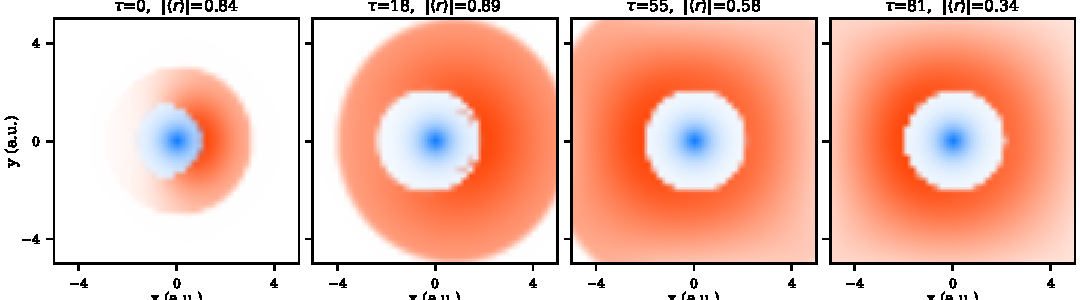
\includegraphics[width=\textwidth]{fig_li_snaps.pdf}
\caption{\DIFaddFL{The same run as Figure~\ref{fig:liwrap}, seen in space: sections through the kernel at
four times, with the Li$^+$ core in blue and the arriving charge in red, intensity following
density on its own territory. At $\tau=6$ the arriving charge is a half-shell on one side and
there is no shell anywhere; it then sweeps around the core and closes into one. The core is
unchanged throughout --- centred, compact, holding exactly its two charges at
$r_{50}=0.66$~a.u. --- and at no time does the arriving charge enter it. This is what the
non-overlap condition does in practice: the interface moves only where a domain's amplitude
locally wins, and against a formed core it does not, so the only direction available to the
incoming charge is around.}}
\label{fig:lisnaps}
\end{figure}

\paragraph{The shell radius is an attractor, not a memory of the seed.} \DIFadd{One objection to a
demonstration of this kind is that the interface may simply have stayed where it was put. The
three-dimensional runs seed the partition at a radius $R_0$ through the core's initial extent, and
that seeding fixes nothing thereafter: the interface is free, and where it settles is an output. The
test is to vary $R_0$ and see whether the outcome is the same, and it is. Seeded at $R_0=1.0$ the
shell settles at $2.139$~au; seeded at $R_0=1.6$ it settles at $2.153$~au }\DIFaddend --- \DIFdelbegin \DIFdel{the floor that sets
the level }\DIFdelend \DIFaddbegin \DIFadd{a spread of $0.7\%$ on
a quantity nothing in the calculation prescribes. A boundary that merely remembered its seed would
have kept the $60\%$ difference it was given.
}

\DIFadd{The same runs give the domain charges, which are the other thing to check: the core holds $2.02$
charges at mean radius $0.76$~au and the arriving electron $1.07$ at mean radius $4.0$~au, so the
two-domain structure is what the relaxation maintains and not an artefact of how it was started.
}

\DIFadd{Against the radial solver the three-dimensional shell sits $12\%$ high }\DIFaddend --- \DIFaddbegin \DIFadd{$2.15$~au against
$1.91$~au for the same configuration in Section~\ref{sec:TEexplicit}. That offset is accounted for
and is not evidence of disagreement: these runs use a kernel softened to $\varepsilon=2h$, which
leaves the well some $9\%$ too shallow at lithium's $1s$ peak, and a shallower well gives a wider
shell. What the three-dimensional runs are offered for is the mechanism, not the radius.
}

\DIFadd{For Be the balanced condition decides alone, and it gives $2{+}1{+}1$: the row's capacity is
$8$, two cap-4 shells, and the two charges of the period take one place in each rather than two
in one. The energy prefers otherwise, and by a converged margin: on a step ladder flat from
$16\,000$ steps to $64\,000$, $2{+}2$ comes out at $-14.8934$ against $-14.6028$ for $2{+}1{+}1$,
lower by $0.291$~Ha, or $7.9$~eV. That is not a competing verdict but the monotonicity stated
above, seen at one element. The three candidates fall in order of compactness --- a single
$4$-shell at $-18.893$ ($28.8\%$ too deep), $2{+}2$ at $-14.893$ ($1.54\%$ too deep), $2{+}1{+}1$
at $-14.603$ ($0.44\%$ short) --- so the lower energy is reached by over-binding }\emph{\DIFadd{past}} \DIFadd{the
reference, and $2{+}1{+}1$ is at once the least bound of the three and the closest to it.
Beryllium is thus the whole pattern in miniature, and it is the reason the energy is not allowed
to choose. Nor do we read the outer
two charges as a $2s^2$ pair: row~2 has capacity $8=4{+}4$ and no pair
(Section~\ref{sec:twoeight}), so they are two of a tetrahedron's four places, and whether they
settle antipodally within it is the ambiguity noted below. For B and C the closure condition is
doing the work, since the energy alone would continue to fill the inner shell.
}

\paragraph{Where the construction is incomplete.} \DIFadd{Two limits should be stated plainly, since
neither is apparent from the results above.
}

\emph{\DIFadd{The build-up is exhibited as a dynamics only at its first step.}} \DIFadd{Figures~\ref{fig:liwrap}
and~\ref{fig:lisnaps} add one charge to Li$^+$ and follow it, and what they illustrate is one of
the two cases: the }\emph{\DIFadd{opening of a new shell}}\DIFadd{, the arriving charge finding the inner shell
closed and taking up position outside it. The other case --- a charge joining a shell already
open, which must then rearrange to share it --- is not shown. Beryllium is its first instance,
$2{+}1$ going to $2{+}1{+}1$ as the arriving charge takes a place in the second cap-4 shell
rather than joining the resident one, and it is the natural next step. Nothing here carries the construction further up the row. What supports
Li through C is the comparison of }\emph{\DIFadd{converged}} \DIFadd{configurations reported above --- the energy
selecting correctly among those a build-up would leave available --- which is a statement about
the outcome, not a simulation of the process. We therefore offer the dynamic Aufbau as
something the model makes explorable, opened at the first step, rather than as a mechanism
already carried through the table.
}

\emph{\DIFadd{And from nitrogen onward even the static rule is undetermined.}} \DIFadd{A shell holding two
charges may be a closed antipodal pair or a half-filled tetrahedron, and no }\emph{\DIFadd{energy}}
\DIFadd{comparison in the present model distinguishes them; the build-up then either opens a spurious
further shell or over-fills the existing one. We report the rule as established for Li through C
and open beyond, rather than extrapolate it.
}

\DIFadd{It is worth recording that a constraint the build-up does not currently use can settle that
choice, and it is not an energy criterion. Take potassium and calcium, where the same ambiguity
recurs one period up: the nineteenth and twentieth charges are either a closed pair or two of a
tetrahedron's four places. On the second reading the tetrahedron completes at $Z=22$, leaving
$36-22=14$ charges to the next closure --- }\DIFaddend and \DIFdelbegin \DIFdel{$E_{\rm val}$ the RealQM valence energy from }\DIFdelend \DIFaddbegin \DIFadd{$14 \equiv 6 \pmod 8$, which by
Section~\ref{sec:twoeight} cannot be composed from octets and at most one pair. The reading is
excluded, and calcium's pair must be closed. So the parity rule has force the
local energies lack: it rules out completions that cannot reach a closed shell. Whether feeding
it to the build-up as a filter carries the construction past carbon we have not tested, and it
would not derive the capacities --- it presupposes them --- but it is the obvious next thing to
try, and it is the reason we call the rule open rather than refuted. It follows that there is no break at $Z=18$ in the Aufbau, which stops far
earlier; $Z=18$ bounds the }\emph{\DIFadd{energies}}\DIFadd{, whose configurations come from the capacities and
the balanced rule.
}

\subsection{Two numbers, not four: the pair and the octet}\label{sec:twoeight}

\DIFadd{This model has }\emph{\DIFadd{two}} \DIFadd{primitive packings, and there is no third. They are the
}\emph{\DIFadd{antipodal pair}}\DIFadd{, $2$, and the }\emph{\DIFadd{tetrahedron}}\DIFadd{, $4$ --- }\DIFaddend the \DIFdelbegin \DIFdel{spherical
pseudo-kernel solve, the valence held outside the core radius $r_c$ by a Neumann
boundary $u'(r_c)=0$ }\DIFdelend \DIFaddbegin \DIFadd{close-packings of two and of
four unit charge clouds on a shell under Coulomb repulsion, both measured above and neither
imported. Eight is not a third primitive: it is $4{+}4$, two dual tetrahedra on the corners of a
cube, a single shell of eight over-binding by $9$--$22\%$ }\DIFaddend (Section~\DIFdelbegin \DIFdel{\ref{sec:radialsolver}). For period~2 the floor is the two-electron He-like core, known analytically as $-Z^2+\tfrac58 Z-0.158$; for periods 3--6 it is taken from
reference data}\DIFdelend \DIFaddbegin \DIFadd{\ref{sec:packing}). Every
shell in every row of the table is a pair or an octet, repeated; in the atom the tetrahedron
never closes a shell on its own, appearing only doubled.
}

\DIFadd{That last fact has a geometric reason, and it is the strongest leg the capacity argument has, so it
should be stated here rather than left to Section~\ref{sec:discussion} where it is developed}\DIFaddend . A
single \DIFdelbegin \DIFdel{$r_c$ per period and block sets the level from one reference
energy }\DIFdelend \DIFaddbegin \DIFadd{tetrahedron has $T_d$ symmetry and }\emph{\DIFadd{no inversion centre}}\DIFadd{: it is directional, and a
directional shell is a reactive one }\DIFaddend --- \DIFdelbegin \DIFdel{the alkaline-earth valence energy for the $s$-block, the noble-gas valence
energy for the $p$-block }\DIFdelend \DIFaddbegin \DIFadd{those four vertices are carbon's four bond directions. Its
}\emph{\DIFadd{dual}}\DIFadd{, the tetrahedron inverted through the centre, is a distinct arrangement, and the union
of the two is the cube, $O_h$, which }\emph{\DIFadd{is}} \DIFadd{centrosymmetric. A closed shell must be spherically
symmetric, and of the two only the cube is. So $4$ cannot close and $8$ can, and the sequence stops
there: the cube admits no further dual, being already its own inversion. The pair is centrosymmetric
from the outset, which is why it closes at $2$ without doubling at all. Two filled packings and no
third, for that reason.
}

\paragraph{Two doublings, and they are not the same doubling.} \DIFadd{The word is now carrying two jobs and
they should be kept apart. The }\emph{\DIFadd{octet}} \DIFadd{doubling is a tetrahedron together with its dual, inside
one shell, giving the cube $4{+}4=8$; it is explained by the inversion argument just given. The
}\emph{\DIFadd{period}} \DIFadd{doubling is a whole capacity $\mathrm{cap}(n)$ serving two consecutive rows }\DIFaddend ---
\DIFdelbegin \DIFdel{so the remaining sixatoms of each period are predictions. }\DIFdelend \DIFaddbegin \DIFadd{$8,8$ then $18,18$ then $32,32$ --- and it is not explained by inversion or by anything else here;
it is the open item, with only the areal argument below pointing at it. The two concern different
objects, one within a shell and one across rows, and an explanation of the first is not a
down-payment on the second.
}\DIFaddend 

\DIFdelbegin \DIFdel{TABLE }\DIFdelend \DIFaddbegin \DIFadd{The capacity unit is therefore $8$, and the table is at its shortest written in that unit }\DIFaddend ---
\DIFdelbegin \DIFdel{Frozen-core total energies eq: frozencore for representative main-group atoms versus reference. Every atom with }\DIFdelend \DIFaddbegin \DIFadd{$2\mid 8\mid 8\mid 2{+}8{+}8\mid 2{+}8{+}8\mid 8{+}8{+}8{+}8\mid 8{+}8{+}8{+}8$, seventeen
shells rather than thirty-one. The spherically homogenised calculations cannot use it, however:
eight charges smeared onto one sphere sit closer to the kernel than $4{+}4$ spread over two
radii and over-bind by $9$--$22\%$ (Section~\ref{sec:packing}). So each octet is }\emph{\DIFadd{realised}}
\DIFadd{in the radial model as two shells of four. That is a cost of the homogenisation
(Section~\ref{sec:radialsolver}), not a claim that the octet is two concentric objects.
}\DIFaddend 

\DIFdelbegin \DIFdel{Table~\ref{tab:frozencore} reports the absolute total energies: every main-group atom
from $Z=11$ (Na) to $Z=86$ (Rn) is within $0.5\%$, periods 4--6 within $0.05\%$. This
precision is }\DIFdelend \DIFaddbegin \DIFadd{It should be said at the outset how far this is from the $s,p,d,f$ picture, because the
agreement on row lengths can disguise it. That picture has four capacities, $2,6,10,14$,
being the spherical-harmonic counts $2(2\ell+1)$ for $\ell=0,1,2,3$. }\emph{\DIFadd{Three of those four
never occur here.}} \DIFadd{There is no $6$ and no shell of six; no $10$ and no shell of ten; no $14$.
They are not present as approximations, nor as limits, nor under other names --- the packing
simply has no such arrangement, and a row of length $8k{+}4$ or $8k{+}6$, which is what a
sub-shell of six or ten would require, cannot be composed at all. What survives is the
number $2$, and even that survives as a different object: not the $\ell=0$ harmonic but two
unit charges at opposite poles, geometry rather than angular momentum.
}

\DIFadd{So the two accounts are not variants of one scheme. They agree on the row lengths and on
nothing beneath them, and what lies beneath is what bonding geometry reads.
}

\paragraph{Where the capacities come from.} \DIFadd{Nothing is imported. The basic filled units are the
}\emph{\DIFadd{antipodal pair}}\DIFaddend , \DIFdelbegin \DIFdel{as itmust be
}\DIFdelend \DIFaddbegin \DIFadd{$2$, and the }\emph{\DIFadd{dual tetrahedra}}\DIFaddend , \DIFdelbegin \DIFdel{carried by the floor }\DIFdelend \DIFaddbegin \DIFadd{$8=4{+}4$, each established above and
neither imported. Composing rows from those two:
}


\DIFadd{TABLE }\DIFaddend --- \DIFdelbegin \DIFdel{the valence is a small fraction
of the deep total, so once the core is referenced the absolute total follows. The substantive content is therefore not the absolute number but $E_{\rm val}$ and its
variation across the table}\DIFdelend \DIFaddbegin \DIFadd{table without caption
}


\DIFadd{Every row length and every closure of the table decomposes into the two packings and nothing
else, with no appeal to an orbital count. The last two columns are of course not independent
evidence: the closures are the partial sums of the lengths and the lengths are the first
differences of the closures, so reproducing one is reproducing the other, and we count it once. The claim is one of decomposition, and the distinction
matters: that a row of length $18$ }\emph{\DIFadd{is}} \DIFadd{a pair and two octets is established below; that the
third row }\emph{\DIFadd{has}} \DIFadd{length $8$ and the fourth $18$ is not derived here. The period lengths are
supplied to the configuration generator, not produced by it, and the doubling of each capacity
across two periods remains open (Section~\ref{sec:discussion}). On this reading $18$ is not $9{+}9$ but $2{+}8{+}8$ --- a pair
together with two octets --- which is also how the fourth row divides in fact, two elements then
sixteen; and $32$ is four octets outright.
}

\DIFadd{That this closes is not the triviality that any even number is a multiple of eight plus a
remainder. The remainder is constrained: the model possesses a pair and an octet and nothing
between them, so a row of length $8k+4$ or $8k+6$ would need half an octet or three quarters of
one, and could not be composed at all. What holds instead is
}\[
2n^2 \equiv \begin{cases} 2 \pmod 8, & n \text{ odd},\\ 0 \pmod 8, & n \text{ even},\end{cases}
\]
\DIFadd{since $n=2m$ gives $2n^2=8m^2$, while $n$ odd gives $n^2\equiv1\pmod 4$. The remainder is only
ever $0$ or $2$ --- never $4$ or $6$ --- so every capacity, at every $n$, is a whole number of
octets carrying at most one pair, and the pair appears exactly when $n$ is odd. The leading $2$
of rows 4}\DIFaddend , \DIFdelbegin \DIFdel{which RealQM supplies and which the ionization energies of
Section~\ref{sec:ie} test directly. }\DIFdelend \DIFaddbegin \DIFadd{5, 8 and 9 is therefore not an irregularity to be excused but the parity of $n$.
}\DIFaddend 

\DIFdelbegin \DIFdel{Two points sharpen the picture. }\DIFdelend \DIFaddbegin \DIFadd{It should be said plainly what this does and does not do. Written in the model's units the
capacity is $8\lfloor n/2\rfloor\lceil n/2\rceil + 2(n\bmod 2)$, which is identically $2n^2$ --- a
restatement of the shell fill, not a derivation of it. What it buys is provenance: the numbers are
reached from the pair and the octet without the hydrogenic count entering, and are }\emph{\DIFadd{then}}
\DIFadd{found to agree with it. The content lies in the constraint above, that the remainder can only be
$0$ or $2$, and in what follows.
}

\DIFadd{The capacities are better given as a construction than as a formula, and the construction needs
no notation at all: }\emph{\DIFadd{to pass from one shell to the next, add $\lceil n/2\rceil$ octets and
flip the pair on or off}} \DIFadd{--- on when $n$ becomes odd, off when it becomes even. Every ingredient of
that step is one of the two measured units, and no quantity from outside the model enters at any
point. In octets the
increments run $1,1,2,2,3,3,4,\dots$ and the pair alternates present/absent, giving
}\[
2 \;\to\; 8 \;\to\; 18 \;\to\; 32 \;\to\; 50 \;\to\; 72 \;\to\; 98 \;\to\; \dots
\]
\DIFadd{with first differences $6,10,14,18,22,26,30$ --- arithmetic, second difference a constant $4$.
That is why the growth of the table looks even rather than lurching: the octet increment advances
by one every }\emph{\DIFadd{two}} \DIFadd{shells, and the tapering a reader sees in the sequence of closed shells is
exactly $\lceil n/2 \rceil$.
}

\DIFadd{The repetition of each capacity across two rows is visible in all of this, and in three equivalent
guises: each capacity serves two rows; $\lfloor n/2\rfloor$ takes each value twice in the closed
form; and $\lceil n/2\rceil$ takes each value twice in the step. These are one fact seen three
ways, not three facts. It is worth noting how narrow that leaves the open
question: the doubling is now contained entirely in a single ceiling function, so what wants
explaining is precisely why the octet increment advances once per two shells rather than once per
shell.
}

\DIFadd{It is worth seeing what the alternative would be, since a table without the doubling is perfectly
thinkable: one period per radial shell, each filled to its capacity $2n^2$. Rows would then run
$2,8,18,32,50,\dots$ and the closures would be their partial sums,
}\[
2,\;10,\;28,\;60,\;110,\;182,\;280 ,
\]
\DIFadd{against the actual $2,10,18,36,54,86,118$. The two agree exactly for helium and neon and part
company at the third closure --- argon at $18$ where the undoubled table would close at $28$. So the
doubling is not a decorative feature of the sequence: it is precisely what makes the periodic table
differ from the one radial filling alone would give, and it does so from the third row on.
}

\DIFadd{It should be said that the orbital account does not explain this either. There, row~3 stops at $18$
because $3d$ does not fill until row~4, which is the $(n{+}\ell)$ ordering --- and that ordering,
$4s$ before $3d$ in particular, has no first-principles derivation
(Section~\ref{sec:intro}). The departure from the undoubled table is encoded in an empirical rule
rather than derived from one. Both accounts therefore face the same open question; what differs is
that a packing account poses it as a question about }\emph{\DIFadd{radius}}\DIFadd{, where an answer could come from
geometry, rather than as a filling order.
}

\DIFadd{That answer is not in hand, but it is worth recording where it would have to come from,
because the number two is not free. Suppose each capacity is used $k$ times. The growth of
capacity }\DIFaddend \emph{\DIFdelbegin \DIFdel{Period~2 is the exception}\DIFdelend \DIFaddbegin \DIFadd{per period}\DIFaddend } \DIFdelbegin \DIFdel{: its He floor is so
shallow that the valence is a large fraction of the total, and the absolute error rises
to }\DIFdelend \DIFaddbegin \DIFadd{is then the $k$th root of its growth per shell, and at $k=2$ that
comes out exactly
}\[
\sqrt{\frac{\mathrm{cap}(n{+}1)}{\mathrm{cap}(n)}} \;=\; \frac{n{+}1}{n},
\]
\DIFadd{since $\mathrm{cap}\propto n^2$ --- the ratios being $2,\ \tfrac32,\ \tfrac43,\ \tfrac54,\dots$
against $4,\ 2.25,\ 1.78,\ 1.56,\dots$ per shell. So $k=2$ is the value that converts the
quadratic growth of the capacity into the }\emph{\DIFadd{linear}} \DIFadd{ratio $(n{+}1)/n$. If the capacity is an
area, going as $r^2$ with $r$ advancing by one unit per period, then two periods are what an
areal shell costs, and the doubling is the exponent in $r^2$ rather than an extra rule. No other
$k$ does this: $k=3$ gives $1.59,\ 1.31,\ 1.21$, smoother still, so a preference for smoothness
alone would drive $k$ upward without limit, and it is the dimensionality that picks out two.
}

\DIFadd{Stated at its sharpest, the thought is this. With one unit of radius per shell, $r_n=n$, the radius
grows between shells by the factor $(n{+}1)/n$, and an areal capacity grows by the square of that. If
each period contributes }\emph{\DIFadd{one}} \DIFadd{such factor, then a capacity carrying }\emph{\DIFadd{two}} \DIFadd{of them takes two
periods, and the number of periods per shell is the exponent in the capacity's scaling with radius
--- }\DIFaddend $2$ \DIFaddbegin \DIFadd{because a shell is a surface, and it would be $3$ for a capacity going as $r^3$.
}

\textbf{\DIFadd{But this does not derive the doubling, and we should not pretend otherwise.}} \DIFadd{Write the
per-period growth as $(\mathrm{cap}(n{+}1)/\mathrm{cap}(n))^{1/k}=((n{+}1)/n)^{2/k}$ and require it
to be one factor of $(n{+}1)/n$: that requires $2/k=1$, which is $k=2$. The premise ``one factor of
$r$ per period'' is therefore }\emph{\DIFadd{equivalent}} \DIFadd{to the conclusion, given $\mathrm{cap}\propto r^2$.
It is the doubling written multiplicatively, not an independent assumption from which the doubling
follows.
}

\DIFadd{What the argument does, then, is relocate the question rather than answer it: from }\emph{\DIFadd{why does
each capacity serve two periods}} \DIFadd{to }\emph{\DIFadd{why does each period correspond to one factor of $r$}}\DIFadd{. We
record it because the second form is a question about radial geometry, where an answer might come
from the packing, rather than a question about an integer sequence, where it cannot; and because the
conditional has content even so --- granted the linking premise, the dimensionality fixes the
multiplicity at two rather than at any other number. But the antecedent is the thing to be explained,
and the doubling remains open.
}

\DIFadd{There is a better reason than circularity for abandoning this route, and it comes from the model's
own radii. The thickness of a shell is set by the net attraction it feels from the kernel. Measured
on argon, with $Z_{\rm eff}=Z$ less the charge inside, the thicknesses $0.626$, $1.224$, $2.601$~au
of the second, third and fourth shells follow $d_n \propto n/Z_{\rm eff}$ to within $2$}\DIFaddend --\DIFdelbegin \DIFdel{$3\%$ for the lightest $p$-block atoms (B, F, Ne; C, N,
O remain near $1\%$).
There the all-electron solve of Table~\ref{tab:TE} is actually more accurate, and the
two methods cross over cleanly }\DIFdelend \DIFaddbegin \DIFadd{$4\%$ }\DIFaddend ---
\DIFdelbegin \DIFdel{explicit wins for period~2 (shallow floor), frozen
core wins decisively for periods 3+ (e.g.\ Si: $+0.3\%$ frozen versus $+4.6\%$
explicit). }\DIFdelend \DIFaddbegin \DIFadd{which is the hydrogenic law, $r_n \propto n^2/Z_{\rm eff}$ differentiated, and it is obeyed by a
solver fitted to nothing. Summing the thicknesses then gives the radius, and the two together give
the shell's volume.
}

\DIFadd{Carried through, that chain }\emph{\DIFadd{does}} \DIFadd{deliver the capacity. With $d_n\propto n/Z_{\rm eff}$ and
$r_n\propto n^2/Z_{\rm eff}$ the ratio is $r_n/d_n \propto n/2$, so a shell of volume $4\pi r_n^2d_n$
filled with charges of volume ${\sim}d_n^3$ holds
}\[
N_n \;=\; \frac{4\pi r_n^2 d_n}{d_n^3} \;=\; 4\pi\Big(\frac{r_n}{d_n}\Big)^{\!2} \;\propto\; n^2 ,
\]
\DIFadd{the constant coming out $\pi$ against the required $2$, a factor $1.6$ which is within the measured
ratio of charge size to shell thickness ($1.3$--$1.8$). So $2n^2$ per shell is recoverable from the
geometry.
}

\DIFadd{In that }\DIFaddend \emph{\DIFdelbegin \DIFdel{The transition elements are absorbed into the floor}%DIFDELCMD < \MBLOCKRIGHTBRACE%%%
\DIFdel{: }\DIFdelend \DIFaddbegin \DIFadd{idealised}} \DIFadd{form the chain excludes the doubling, and it is worth seeing why before
reading anything into it. Since $r_n\propto n^2/Z_{\rm eff}$ and $d_n\propto n/Z_{\rm eff}$ carry the
same $Z_{\rm eff}$, it cancels: $r_n/d_n=n/2$ exactly, with no dependence on $Z$ at all. The capacity
is then a pure function of $n$, no two shells can share one, the rows run $2,8,18,32,50$ and the
closures are $2,10,28,60$ --- the undoubled table.
}

\textbf{\DIFadd{But the measured ratios do not behave that way, and the departure is in the direction the
doubling needs.}} \DIFadd{On argon the four shells give $r_n/d_n = 0.50,\ 0.90,\ 1.21,\ 1.31$ against the
idealised $0.50,\ 1.00,\ 1.50,\ 2.00$: the ratio }\emph{\DIFadd{saturates}}\DIFadd{. The corresponding capacities
$4\pi(r_n/d_n)^2$ are $3.1,\ 10.2,\ 18.4,\ 21.6$ --- and the last two are nearly equal. Two
consecutive shells of the same capacity is exactly what the repetition of a row capacity requires,
and the idealised form excluded it only by letting $Z_{\rm eff}$ cancel.
}

\DIFadd{This also puts the row lengths in reach as }\DIFaddend a \DIFdelbegin \DIFdel{period-4
$p$-block atom sits on an }%DIFDELCMD < [%%%
\DIFdel{Ar}%DIFDELCMD < ]%%%
\DIFdel{$3d^{10}$ core, a period-6 oneon an }%DIFDELCMD < [%%%
\DIFdel{Xe}%DIFDELCMD < ]%%%
\DIFdel{$4f^{14}5d^{10}$
core.
These buried shells are not resolved; they serve as the reference level, which is
exactly their physical role}\DIFdelend \DIFaddbegin \emph{\DIFadd{capacity}} \DIFadd{question rather than a filling one. The
second shell above houses about $8$ to $10$ charges, not $18$: at the radius the screening has so far
produced, there is not room for $18$. On that reading the third row is $8$ and not $18$ because the
shell available cannot hold $18$ yet, and the capacity rises to $18$ only when the radius has grown
enough --- which is the saturation above, seen from the other side}\DIFaddend .

\DIFdelbegin \DIFdel{Table~\ref{tab:master} collects the full main-group result}\DIFdelend \DIFaddbegin \DIFadd{We put this forward as the most promising route we have and not as a result, because it is one atom,
and because the occupancies here are supplied: the solver was told to place $2{+}4{+}4{+}4{+}4$, so
the geometry relaxed around a filling it did not choose, and a capacity read off that geometry cannot
be independent of it. What would settle it is the same measurement across atoms and across candidate
fillings }\DIFaddend --- \DIFdelbegin \DIFdel{total energy and first
ionization energy, each with its error, for every atom from Li to Rn. It is }\DIFdelend \DIFaddbegin \DIFadd{does $4\pi(r/d)^2$ track $2,8,8,18,18$, repetitions and all, or does it track $2n^2$?
That computation has since been made, on four atoms and three candidate fillings, and it does not
settle the question so much as bound it. Tested shell by shell against the occupancy it was given,
the pair-and-octet filling is the more self-consistent of the two we use: the mean departure of
$4\pi(r/d)^2$ from the occupancy it is supposed to hold is $0.55$, against $1.34$ for the balanced
cap-4 rule, while a filling that buries a pair }\emph{\DIFadd{inside}} \DIFadd{the fourth row ---
$2{+}8{+}8{+}2{+}8{+}8$ for krypton --- fails outright, a two-charge shell at $r/d=3.7$ returning a
capacity of $175$. That comparison assumes no answer: it asks of each candidate filling only whether
the geometry it relaxes into can hold what it was given.
}

\DIFadd{Its weight should not be overstated. The innermost shell is an }\emph{\DIFadd{identity}} \DIFadd{and not a
measurement --- with $r_{\rm in}=0$ }\DIFaddend the \DIFdelbegin \DIFdel{periodic table in RealQM: total energies within $1\%$ for $Z\ge 11$ (}\DIFdelend \DIFaddbegin \DIFadd{mid-radius is half the thickness, so $r/d=1/2$ and
$4\pi(r/d)^2=\pi$ exactly, which is where the factor $\pi$ against the required $2$ above comes from
--- and the outermost shell's thickness is set by the box rather than by a relaxed interface. Removing
both leaves three informative shells for }\DIFaddend the \DIFdelbegin \DIFdel{period-2
$p$-block the }\DIFdelend \DIFaddbegin \DIFadd{pair-and-octet rule, and krypton's third shell misses by
a factor of two. We therefore record the capacity estimate as an }\emph{\DIFadd{anticipation}} \DIFadd{of the filling at
larger $Z$, to be confirmed or refuted when the build-up of Section~\ref{sec:aufbau} is carried past
carbon, and not as a derivation of it. The true filling can come only from the build-up; capacity is
what lets us guess it where the build-up does not yet reach.
}

\paragraph{What closure requires, and what precedes it.} \emph{\DIFadd{Closure is exhaustion of a row's
capacity}}\DIFadd{, and that is what this construction means by a noble gas: at $Z=2,10,18,36,54,86,118$ ---
the partial sums of $2,8,8,18,18,32,32$ --- every shell the period provides is full, so an arriving
charge has no vacant site at that radius and must open a new shell further out, which is what begins
the next period. Rubidium opening a shell outside a complete fourth row is the mechanism, and it
requires nothing about the shape of the outer layer.
}

\DIFadd{In the second and third rows closure can equally be stated as a completed outermost octet, because
there the row }\emph{\DIFadd{is}} \DIFadd{one octet and the two statements coincide. A closed outermost octet is
reached only when every shell inside it is itself complete, at }\DIFaddend $2$ \DIFdelbegin \DIFdel{--$6\%$ exception), }\DIFdelend \DIFaddbegin \DIFadd{or at $8$; so for those rows, since
the outermost octet is completed only at a closure, }\emph{\DIFadd{no atom can carry a complete outermost
octet without being a noble gas}}\DIFadd{, and the octet outermost is unavailable to anything else. From the
fourth row on the two part company --- the row is a pair and two octets, and the pair may stand
outside --- so it is capacity exhaustion and not the outer layer's shape that carries the account
there. The next paragraph gives krypton in both of the fillings we use, neither of which puts an
octet outside.
}

\DIFadd{One limit of this should be said plainly. What is explained here is }\emph{\DIFadd{where}} \DIFadd{the noble gases
fall in the table, not }\emph{\DIFadd{why they are unreactive}}\DIFadd{: the account is structural --- a closed row
offers no vacant site --- and not energetic. The ionisation energies that would carry inertness are
not reported in this paper at all (Section~\ref{sec:limitations}); ionization and excitation are
left to a companion article.
}

\DIFadd{The converse does not hold, and the reason is worth setting out fully rather than hiding. Helium's
shell }\emph{\DIFadd{is}} \DIFadd{the pair, so it closes at $2$ and never has an octet outside. The fourth and fifth
rows fail for a different reason, and krypton shows it twice over. Its row }\emph{\DIFadd{is}} \DIFadd{complete --- the
capacity is $18$ and all eighteen charges are present, so the closure $2{+}8{+}8{+}18=36$ is exact
--- but the outermost eight is not realised as $4{+}4$ under either filling rule we use. The balanced
cap-4 rule of Section~\ref{sec:packing} has period-4 caps $4{+}4{+}4{+}4{+}2$, the pair }\emph{\DIFadd{last}}\DIFadd{,
and so returns
}\[
\mathrm{Kr} \;=\; 2{+}4{+}4{+}4{+}4\;|\;4{+}4{+}4{+}4{+}2 ,
\]
\DIFadd{with the cap-2 pair outermost and the two octets inside it. The configurations actually used for the
fourth row (Table~\ref{tab:TE4}) come from the ionisation order instead, and give
}\[
\mathrm{Kr} \;=\; 2{+}4{+}4{+}4{+}4\;|\;4{+}3{+}3\;|\;2\;|\;3{+}3 ,
\]
\DIFadd{grouped as $[\mathrm{Ar}]$, then $3d$, then the $4s$ pair, then $4p$ --- so the outer group is
$3{+}3$ and the outermost octet is $2{+}3{+}3$ across three shells. Neither is two tetrahedra.
}

\DIFadd{This is not merely an artefact of the rules. Krypton is $[\mathrm{Ar}]\,3d^{10}4s^24p^6$, so its
outermost eight is a }\emph{\DIFadd{pair and six}} \DIFadd{in the orbital account as well; the eight at the outside of
a fourth-row noble gas is not a $4{+}4$ object in any picture. What closes correctly at $36$ is the
capacity, and that is what the construction of Section~\ref{sec:twoeight} claims. Where the pair sits
radially --- outermost, as the caps place it, or innermost, as the table's own filling order at
potassium and calcium suggests --- is the radial-ordering question raised below, and it is not settled
here.
}

\DIFadd{The build-up makes the approach to closure explicit, and gives the element before each noble gas a
geometry. Filling a row's two tetrahedra evenly, the occupancies run
$1{+}1$, $2{+}1$, $2{+}2$, $3{+}2$, $3{+}3$, $4{+}3$, $4{+}4$: the last step before closure is
always $4{+}3$ --- one tetrahedron complete, the other one vertex short. That is fluorine,
$2{+}4{+}3$, and chlorine, $2{+}4{+}4{+}4{+}3$ (Table~\ref{tab:TE}). So the halogens are not
merely ``one electron short'' as a count; they are short of }\emph{\DIFadd{one tetrahedral vertex}}\DIFadd{, a
definite vacant site next to a filled tetrahedron, and an arriving charge completes the octet by
occupying it. The noble gas is the same structure with that site filled.
}

\DIFadd{The octet rule is then doing far more work than it is usually given. It is not merely the rule
for the second and third rows: it is the unit out of which every later row is built, $18$ being
a pair and two octets and $32$ four octets, rather than capacities of their own.
}

\DIFadd{One caution about that grouping. The homogenised solver returns argon as
$2{+}4{+}4{+}4{+}4$ --- five shells, each owning a disjoint radial interval --- with free
boundaries at $0.249$, $0.875$, $2.099$ }\DIFaddend and \DIFdelbegin \DIFdel{first ionization energies within $10$--$20\%$
for the }\DIFdelend \DIFaddbegin \DIFadd{$4.700$~au, so the four tetrahedra sit at
successive radii in the ratios $2.65$, $2.29$, $2.16$. They are uniformly nested, not paired:
were each octet a cube of eight at one radius, the four would fall into two close pairs, and
they do not. The bracketing of them as $(4{+}4)+(4{+}4)$ is therefore an }\emph{\DIFadd{interpretation}}
\DIFadd{of the counts, not an output of this calculation --- and it could not be an output, since a
radial model cannot place two tetrahedra at a common radius in the first place. Whether the
octet closes as a cube at one radius or as two nested tetrahedra is a three-dimensional
question, and it is open here.
}

\DIFadd{Because the octet is built as $4{+}4$, the leading octet of rows 6 and 7 may equally be written
as two tetrahedra, $32=(4{+}4)+8+8+8$. The count is unchanged; what is open is whether that
first group closes into a cube or remains two tetrahedra, and the arithmetic cannot decide it.
This is worth recording because it is precisely the region the orbital account assigns to the
$f$ sub-shell, so it is where the two decompositions would be distinguishable if anything
distinguishes them.
}

\DIFadd{The disagreement with the orbital account is the same at every row length, and it is a
disagreement about decomposition rather than about number. Where that account makes the octet
$2{+}6$, an }\DIFaddend $s$ \DIFdelbegin \DIFdel{-block and the heavier }\DIFdelend \DIFaddbegin \DIFadd{pair and three }\DIFaddend $p$ \DIFdelbegin \DIFdel{-block, with the light }\DIFdelend \DIFaddbegin \DIFadd{lobes, this one makes it $4{+}4$; where it makes the fourth
row $2{+}10{+}6$, a pair with five $d$ and three }\DIFaddend $p$\DIFdelbegin \DIFdel{-block under-binding (}\DIFdelend \DIFaddbegin \DIFadd{, this one makes it $2{+}8{+}8$, a pair and
two octets; where it makes the sixth $2{+}14{+}10{+}6$, this one makes it $8{+}8{+}8{+}8$. Both
give $8$, both give $18$, both give $32$. What differs is what the eight, the eighteen and the
thirty-two are }\emph{\DIFadd{made of}}\DIFadd{, and that is what bonding geometry reads.
}

\DIFadd{Two regularities are in play here and should not be run together. The capacities go as $2n^2$
and decompose as above; separately, each capacity serves }\emph{\DIFadd{two}} \DIFadd{rows, all but the first.
The latter is not derived here, and it is worth stating precisely what is missing, because the
usual phrasing --- ``why does each capacity repeat?'' --- points at the wrong place. The
repetitions need no account; what needs one is the }\emph{\DIFadd{growth}}\DIFadd{. Reading the table as a sequence
of increments $2,8,8,18,18,32,32$, an increment is used twice and then grows, so there are two
questions: why after exactly two uses, and why to the next capacity rather
than to anything else. The second is the sharper, since a third increment of $18$ would carry
$54$ to $72$, and $72$ is itself a capacity --- so the alternative is not arithmetically
forbidden, merely not what happens.
}

\DIFadd{It should also be said that the leftover pair at odd $n$ may not be one phenomenon. At $n=1$
there are no octets for it to be left over from: the pair is the entire shell, it is the
innermost and smallest, and ``only two fit at that radius'' is at least available as an
explanation there. At $n=3$ and above the pair sits with octets already present and with radius
in plentiful supply, so nothing of that kind can be doing the work. The two cases share a term in
the parity term and little else, which may be why no single mechanism has accounted for both.
}

\DIFadd{One further caution about the pair at $n=3$. Its radial position and its filling order disagree.
The configuration generator places it outermost, and the table's own filling order places its two
charges first, at potassium and calcium. Both can hold only if a shell that fills early lies
outside shells that fill later --- which is the $4s$-before-$3d$ inversion, and therefore the
same interpenetration that defeats the spherical homogenisation from the fourth row on
(Section~\ref{sec:dblock}). The leftover pair is thus not an independent puzzle; it is where the
d-block problem first shows in the packing account. Read cumulatively, argon, krypton and xenon are one, two and
three copies of the same block, $18=2{+}8{+}8$, so that $Z=18,36,54$ are $1,2,3$ times eighteen
--- a pattern invisible in the orbital decomposition, where the three read $s^2p^6$,
$s^2d^{10}p^6$ and $s^2d^{10}p^6$. It should be said plainly that this is an arithmetic accident
and not a replication principle. Argon's }\emph{\DIFadd{total}}\DIFadd{, $2{+}8{+}8=18$, happens to equal the
}\emph{\DIFadd{next capacity}}\DIFadd{, $2\cdot3^2=18$; the two coincide at argon and nowhere else in the table.
Krypton is therefore argon plus the next shell, not argon twice over, and the pattern duly fails
at radon, which is $86$ rather than $4\times18=72$.
}

\DIFadd{It is worth separating the two things the run is made of, because only one of them wants explaining.
The second and third $18$s are the }\emph{\DIFadd{doubling}}\DIFadd{: rows 4 and 5 carry the same capacity, as rows 2
and 3 do and rows 6 and 7 do. The first $18$ is the coincidence: the first three rows happen to sum
to $2{+}8{+}8=18$, which is $2(1+4+4)=2\cdot3^2$, so the running total after three rows equals the
capacity of the next two. Three equal increments follow, and then row 6 brings $32$ and the run ends.
So the threefold appearance is the doubling plus a single accident at argon, and what is left to
explain is the doubling alone.
}

\DIFadd{We do not claim the familiar $2n^2$ as a result of this model, that count being the hydrogenic
degeneracy; what is claimed is that whatever $2n^2$ is, it is always composable from the pair
and the octet, and in only one way.
}

\paragraph{The same two numbers in the nucleus.} \DIFadd{The pair and the tetrahedron are not features of
the electron. They are the close-packings of }\emph{\DIFadd{unit charge clouds on a shell under Coulomb
repulsion}}\DIFadd{, and that argument is indifferent to what the cloud is or which sign it carries. A
companion article~\mbox{%DIFAUXCMD
\cite{Johnson-RealNucleus} }\hskip0pt\relax %DIFAUXCMD
applies the same model to nuclei, protons and
electrons entered as equal-mass clouds differing only in the sign of the charge, and it builds
them from the same two units: the alpha particle is one electron pair inside one proton
tetrahedron, $2\mid 4$, and $^{16}$O is four such units nested,
$2{+}2{+}2{+}2\mid 4{+}4{+}4{+}4$, its protons therefore two octets.
}

\DIFadd{The first two nuclear magic numbers are $2$ and $8$, and $^4$He and $^{16}$O are the two doubly
magic light nuclei --- exactly the two closures the pair and the octet supply, and exactly the two
that model reaches. Beyond $8$ the two sequences part company: the atomic capacities continue
$18,32,50$ while the magic numbers continue $20,28,50,82,126$, and the latter are not
composable from a pair and octets at all. So what is shared is the }\emph{\DIFadd{unit}}\DIFadd{, not the table
--- the tetrahedron of four unit charges, appearing doubled as the atomic octet and singly as
the alpha. That two systems differing by five orders of magnitude in energy select the same two
arrangements is the strongest indication we have that these capacities are geometry rather than
spectroscopy. We attach no numerical claim to it here: the nuclear binding energies are
provisional, }\DIFaddend the \DIFdelbegin \DIFdel{radial-octet ceiling of Section~\ref{sec:ie}). Total energies and ionization energies
are obtained from their own $r_c$ calibrations (valence-energy and ionization-energy
respectively), so the two error columns reflect two separate fits to one reference each per period. }\DIFdelend \DIFaddbegin \DIFadd{alpha-to-deuteron ratio standing at about $11$ against $12.7$ observed, with
the heavier configurations not yet mesh-converged. Which of the two is the right
reading of the fourth row --- $9{+}9$ or $(2{+}8){+}8$ --- is not settled here; it is worth
recording that they are distinguishable in principle, since only the second is expressible in
the packings this model possesses --- and that the energy does not distinguish them in practice.
Composing krypton as the third row's structure twice over, $2{+}4{+}4{+}4{+}4$ repeated, against
the same $36$ charges packed as $2{+}4{+}4{+}4{+}4\,|\,4{+}3{+}3{+}2{+}3{+}3$, the two differ by
$1.6$~Ha in $2662$, or $0.06\%$; for zinc the corresponding difference is $0.04\%$. Both are a
hundred times smaller than either configuration's distance from the reference, so the comparison
selects nothing. That is the same finding as Section~\ref{sec:aufbau}'s, one row further up: the
energy is not what fixes the structure, and two arrangements of the same charges can sit within
a twentieth of a per cent of each other.
}\DIFaddend 

\DIFaddbegin \subsection{All-electron total energies, periods 1--3}\label{sec:TEexplicit}

\DIFadd{Table~\ref{tab:TE} reports total energies with the balanced cap-4 packing against
near-exact nonrelativistic reference values~\mbox{%DIFAUXCMD
\cite{Chakravorty}}\hskip0pt\relax %DIFAUXCMD
.
}

\paragraph{What the reference column is.} \DIFadd{This deserves saying plainly, because a table of this
shape is naturally read as a comparison against measurement, and it is not one. The
}\emph{\DIFadd{nonrelativistic, stationary-nucleus total electronic energy}} \DIFadd{of an atom is not an
observable. No instrument reads it. What is measured is ionisation energies and spectra; the
reference values are then }\emph{\DIFadd{constructed}} \DIFadd{from those by removing, by calculation, the
relativistic, QED and nuclear-motion contributions that the measurement contains and the
calculation does not. Reference~\mbox{%DIFAUXCMD
\cite{Chakravorty} }\hskip0pt\relax %DIFAUXCMD
is explicit that its energies combine
experimental data with }\emph{\DIFadd{ab initio}} \DIFadd{results, the correlation contribution being obtained by
comparing experiment against relativistic complete-valence-space calculations. Beyond argon the
values available to us are Hartree--Fock level, that is computed outright.
}

\DIFadd{So the comparison here is model against a semi-empirical composite, not model against experiment.
We are not aware of any table of experiment against theory for atomic total energies, and there
cannot straightforwardly be one: the quantity a calculation delivers is not the quantity an
instrument reads, and bridging the two requires exactly the theory under test to supply the
corrections. This does not make the comparison worthless --- the composites are accurate, and
agreement to one or two per cent against them is a real constraint --- but it sets what the
per-cent figures mean. They measure distance from a construction that already contains standard
quantum mechanics, so they cannot be read as a direct verdict of one theory against nature. The
observables this model can be held to without that circularity are of a different kind:
electronegativity ordering (Section~\ref{sec:chi}), shell radii, and geometry.
}



\DIFaddend TABLE --- \DIFdelbegin \DIFdel{Total energies (frozen core) and first ionization energies (pseudo-kernel)for all main-group atoms, with erro
}\DIFdelend \DIFaddbegin \DIFadd{Total atomic energies (balanced cap-4 packing, spherically-homogenised solver) versus near-exact nonrelativist
}\DIFaddend 



\DIFdelbegin %DIFDELCMD < \subsection{Boundary of the spherical model: where radial nesting fails}\label{sec:dblock}
%DIFDELCMD < %%%
\DIFdelend \DIFaddbegin \DIFadd{At the production mesh the mean relative error is $1.6\%$ and the maximum $4.5\%$ (Si, with S at
$4.3\%$), and 13 of the 17 atoms fall within $2.5\%$. Those are the errors }\emph{\DIFadd{of this mesh}} \DIFadd{and
not a converged accuracy: single entries move by a few per cent under refinement, and the movement
is systematic rather than random, so it does not average down over seventeen atoms
(Section~\ref{sec:convergence}). The mean should accordingly be read at the same level as the
entries --- a few per cent --- which is what a 1D radial solve with no basis sets, no antisymmetry
and no two-electron integrals delivers.
}\DIFaddend 

\DIFdelbegin \DIFdel{The spherically-reduced solver is valid exactly as
long as the packing is a nested
sequence of radial shells. This holds for the first three periods --- the first 18
electrons, packed as $2,\ 4{+}4,\ 4{+}4$ }\DIFdelend \DIFaddbegin \DIFadd{We claim no more precision than that, and one entry shows why. Argon's $+0.1\%$ is the closest
agreement in the table and it is not robust: on the same domain, refining the radial mesh to
$N=724$ and $1024$ }\DIFaddend --- \DIFaddbegin \DIFadd{where the $1s$ spans $17$ }\DIFaddend and \DIFdelbegin \DIFdel{through the next two additions
(Z=19, 20).
It breaks at $Z\approx 21$, where the optimal packing ceases to be radially nested: the electrons added thereare }\emph{\DIFdel{not}} %DIFAUXCMD
\DIFdel{the outermost, as shown
model-independently by the ionisation order (they are not the first removed). They
take a more compact, }\emph{\DIFdel{interpenetrating}} %DIFAUXCMD
\DIFdel{arrangement that a model ordering shells
strictly by radius cannot represent, so the radial solver mis-binds and then
diverges. This is not a numerical accident but the
periodic table's first departure
from radial nesting }\DIFdelend \DIFaddbegin \DIFadd{$25$ cells rather than the $10$ it spans at
$N=400$ }\DIFaddend --- \DIFdelbegin \DIFdel{the region conventional orbital theory labels the d-block, though RealQM invokes no angular-momentum orbitals, only packing. Interpenetrating
packings are intrinsically three-dimensional and require the explicit 3D valence
solve. The }\DIFdelend \DIFaddbegin \DIFadd{moves argon to $-511.7$ and $-511.3$~Ha, some $3\%$ }\emph{\DIFadd{under}}\DIFadd{-bound, the two finest
values agreeing with each other to $0.08\%$. Both are step-converged: quadrupling the relaxation at
fixed mesh moves the energy by $0.005$~Ha. So the near-exact argon entry is an artefact of the
production mesh, and nothing here rests on it --- in particular we do not read a }\emph{\DIFadd{sign}} \DIFadd{off
this table, since the sign of argon's error is itself a function of the grid. What the reduction
predicts, and what survives refinement, is under-binding; see
Section~\ref{sec:radialsolver} and Section~\ref{sec:convergence}.
}

\subsection{The fourth row: all-electron energies to krypton}\label{sec:TE4}

\DIFadd{The mesh is chosen by $Z$ rather than held fixed. Since the innermost shell contracts as
$r_{1s}\approx 4.3/Z$, a single $N$ cannot serve the whole table: $N=400$ through argon and $N=800$
from potassium keeps that shell spanned by a comparable number of cells at both ends, which is the
quantity that matters and not the mesh itself. Table~\ref{tab:TE4} reports the fourth row on that
basis --- }\DIFaddend all-electron\DIFdelbegin \DIFdel{results of Section~\ref{sec:TEexplicit} are confined to this
radially-nested regime ($Z\le 18$); the frozen-core results of Section~\ref{sec:frozencore} reach the full main group by absorbing the
$d$- and $f$-blocks into the reference core }\DIFdelend \DIFaddbegin \DIFadd{, bare kernel $-Z/r$, no core radius, no fitted length, nothing adjusted per
element --- so it extends the table of the previous section rather than being obtained by a
different method}\DIFaddend .



\DIFdelbegin %DIFDELCMD < \subsection{Ionization energies}\label{sec:ie}
%DIFDELCMD < %%%
\DIFdelend \DIFaddbegin \DIFadd{TABLE --- All-electron total energies of the fourth row, -- , on the mesh (references as in Table tab:TE ). Configuratio
}\DIFaddend 



\DIFdelbegin \DIFdel{The per-electron route of Section~\ref{sec:model} gives the
first ionization energy
directly as the valence-electron energy, $\mathrm{IE}=|\varepsilon_{\rm valence}|$}\DIFdelend \DIFaddbegin \paragraph{The shell list and the capacity decomposition are different statements.} \DIFadd{These tables
report }\emph{\DIFadd{occupations}} \DIFadd{--- what the filling rule assigns to one atom, shell by shell, as the solver
partitions it. Section~\ref{sec:twoeight} reports }\emph{\DIFadd{capacities}} \DIFadd{--- what a closed shell can hold,
built from the pair and the octet. The two coincide at closed shells and nowhere else:
}\[
\mathrm{He}=2,\qquad \mathrm{Ne}=2{+}8,\qquad \mathrm{Ar}=2{+}8{+}8,\qquad
\mathrm{Kr}=2{+}8{+}8{+}18 ,
\]
\DIFadd{with $18=2{+}8{+}8$ in turn. For every other atom there is no complete octet to display --- the step
before closure is $4{+}3$, one tetrahedron short of a vertex (Section~\ref{sec:twoeight}) --- so the
long lists of twos, threes and fours above are not a competing account of the capacities but the
occupations themselves. We do not write the octets as $(4{+}4)$ in these tables, and the reason is
given below: the solver returns the shells uniformly nested rather than paired, so that bracketing
would assert a structure the computation does not show.
}

\DIFadd{Two things about this row are worth more than its mean error. The first is the }\emph{\DIFadd{sign}}\DIFadd{. Every one
of the eighteen entries is under-bound}\DIFaddend , with no \DIFdelbegin \DIFdel{separate ion calculation. For the two atoms whose valence is a single
outermost shell it is accurate (Table~\ref{tab:ie}): He and Li to ${\sim}1\%$, validating the
method. }\DIFdelend \DIFaddbegin \DIFadd{exception and no trend in $Z$, and under-binding is
what Section~\ref{sec:radialsolver} predicts: the reduction has the pair count right and the pair
geometry wrong, overestimating intra-shell repulsion, and what survives is a deficit of binding. The
third period read the other way at $N=400$, and Section~\ref{sec:TEexplicit} shows why that reading
does not survive refinement --- argon changes the sign of its error between $N=400$ and $N=1024$. So
the fourth row, computed where the $1s$ is resolved, agrees in sign with helium and with resolved
argon, and it is the coarse third-period entries that are the exception.
}\DIFaddend 

\DIFdelbegin \DIFdel{TABLE }\DIFdelend \DIFaddbegin \DIFadd{The second is what the row does }\emph{\DIFadd{not}} \DIFadd{establish. Its configurations are taken from the
ionisation order from scandium onward, because a build-up that adds outward cannot place a charge
inside a shell already occupied, and the fourth row requires exactly that. The energies are
therefore computed in configurations supplied from outside the model, and the accuracy here says
nothing about whether the model would have chosen them. That boundary is the subject of the next
section, and it is a boundary in the }\emph{\DIFadd{build-up}}\DIFadd{, not in the calculation.
}

\paragraph{How much the row depends on that import: almost nothing.} \DIFadd{Since the configurations are
supplied, the obvious question is how much of the error in Table~\ref{tab:TE4} they are responsible
for, and it can be answered by recomputing the row under the model's own rule instead }\DIFaddend --- \DIFdelbegin \DIFdel{First ionization energy as the valence-electron energy (balanced }\DIFdelend \DIFaddbegin \DIFadd{the
balanced }\DIFaddend cap-4 \DIFdelbegin \DIFdel{packing),
versus NIST NIST-ASD }\DIFdelend \DIFaddbegin \DIFadd{filling of Section~\ref{sec:packing}, extrapolated past calcium, in place of the
ionisation order. Both runs at $N=800$, identical step counts, with potassium and calcium as a
control since the two rules return the same configuration there and must therefore agree exactly;
they do. Over $Z=19$--$36$ the mean absolute error is $3.30\%$ under the imported filling and
$3.30\%$ under the model's own, with maxima $6.74\%$ and $6.73\%$; the imported rule is closer for
eleven atoms and the model's own for seven, and every per-atom difference is below $1.3$~Ha except
iron's $4.2$~Ha, with the signs scattered both ways. Selenium, the row's worst entry, moves from
$-6.74\%$ to $-6.73\%$. The row's accuracy therefore does not depend on which rule supplies the
filling: what Table~\ref{tab:TE4} measures is the spherical reduction (Section~\ref{sec:radialsolver}),
not the import}\DIFaddend .

\DIFdelbegin \DIFdel{On a bare nucleus the eigenvalue degrades beyond Li because the outer shell is placed
at over-screened large radius. The pseudo-kernel }\DIFdelend \DIFaddbegin \DIFadd{One further comparison bears on Section~\ref{sec:aufbau} rather than on this row. Partitioning
selenium's thirty-four charges as $2$ plus eight shells of four --- uniform, with no distinct outer
pair and no $d$-shell, so not a configuration either rule produces and not the physical one ---
gives $-2392.1$~Ha against $-2238.1$, some $154$~Ha lower and within $0.3\%$ of the reference instead
of $6.7\%$ away. The more compact and structurally wrong packing wins on energy by a wide margin.
That is the anti-correlation }\DIFaddend of Section~\DIFdelbegin \DIFdel{\ref{sec:twoscale} removes
this: with the core replaced by its reference field and the valence held outside $r_c$
by the Neumann boundary $u'(r_c)=0$, the per-electron route extends across the table. The ionization energy is the }%DIFDELCMD < \emph{%%%
\DIFdel{change}%DIFDELCMD < \MBLOCKRIGHTBRACE %%%
\DIFdel{of energy on removing the outermost
electron --- the prototypical periodic observable }\DIFdelend \DIFaddbegin \DIFadd{\ref{sec:aufbau} appearing again in the fourth row, and it is
the reason the configurations here are not chosen by minimising.
}

\DIFadd{The same ordering holds wherever it is tested, and monotonically in how compactly the charges are
grouped. At equal mesh and step count the error against the reference runs: argon as $2{+}16$,
$+33.6\%$; as $2{+}8{+}8$, $+18.8\%$; as $2{+}4{+}4{+}4{+}4$, $+0.11\%$; neon as $2{+}8$, $+13.7\%$,
as $2{+}4{+}4$, $+2.2\%$. Every grouping over-binds, and the more compact it is the more it over-binds.
This bears directly on the row lengths. The closure an undoubled table would have had at $Z=28$
requires a shell of eighteen, and nickel computed as $2{+}8{+}18$ comes out $+26.5\%$ too deep. So
eighteen in one shell does }\emph{\DIFadd{fit}} \DIFaddend --- \DIFdelbegin \DIFdel{and }\DIFdelend \DIFaddbegin \DIFadd{the calculation converges and returns an energy --- but it
is energetically wrong-signed by a wide margin, which is what one would expect of a packing the
build-up never reaches.
}

\subsection{The shape of the computed field: constant charge per unit radius}\label{sec:psiscale}

\DIFadd{The energies above say nothing about what the solution looks like, and the field turns out to obey a
scaling that nothing in the construction imposes. The solver's charge element is $u^2r^2\,dr$, so $u$
is proportional to $\psi$ itself rather than to the radial function $rR(r)$, and what is measured is
that }\emph{\DIFaddend the \DIFdelbegin \DIFdel{model reproduces its two
defining trends: $\mathrm{IE}$ falls monotonically down every group and rises across
every period. Quantitatively (Table~\ref{tab:ieperiodic}) it }\DIFdelend \DIFaddbegin \DIFadd{charge per unit radius }\DIFaddend is \DIFdelbegin \DIFdel{within $10$}\DIFdelend \DIFaddbegin \DIFadd{the same in every shell and equal to $Z/2$}}\DIFadd{:
}\[
\psi^2 r^2 \;\approx\; \tfrac12 Z ,
\qquad\text{equivalently}\qquad
\psi(r) \;\approx\; \sqrt{\tfrac{Z}{2}}\,\frac{1}{r} .
\]
\DIFadd{The density therefore goes as $Z/r^2$, falling steeply, while the charge in each spherical slab
$dr$ does not vary at all --- not within a shell, and not from one shell to the next.
}

\emph{\DIFadd{Constant within a shell.}} \DIFadd{The coefficient of variation of $ur$ across a shell, with the inner
and outer tenth excluded since $1/r$ cannot hold where the field is finite, is $0.028$ for carbon's
third shell, $0.040$ for krypton's third, $0.090$ for the innermost shell of argon and of krypton,
and $0.18$}\DIFaddend --\DIFdelbegin \DIFdel{$20\%$ for
the $s$-block (alkaline earths to a few percent) and for the heavier $p$-block (periods
5--6, several atoms within a few percent)}\DIFdelend \DIFaddbegin \DIFadd{$0.30$ for the intermediate ones. The outermost shell of each atom gives $1.4$--$2.0$
and is excluded throughout: it runs to the edge of the box, where the field decays to nothing.
}

\emph{\DIFadd{Constant from shell to shell, and equal to $Z/2$.}} \DIFadd{Taken over the interior shells of the
row-structured configurations, $\psi^2r^2$ comes out $9.07$ and $9.62$ for argon against $Z/2=9$, and
$18.22$, $27.27$, $17.97$ for krypton against $Z/2=18$ --- a spread of $3\%$ across argon's shells and
two of krypton's three within $2\%$. Note that it is $Z$ and not a screened charge: the slab density
is set by the bare kernel, with no reference to what lies inside.
}

\emph{\DIFadd{What it fixes.}} \DIFadd{Since a shell's occupancy is the slab density times its thickness, the law
determines the thickness outright,
}\[
d \;=\; \frac{2\,\mathrm{occ}}{Z} ,
\]
\DIFadd{and the measured thicknesses follow it: argon's two inner shells at $0.210$ and $0.810$~au against
$0.222$ and $0.889$ predicted, krypton's three at $0.105$, $0.300$, $0.450$ against $0.111$, $0.444$,
$0.444$. The radius of a shell is then the running sum of those thicknesses, so the whole radial
structure of the atom follows from one constant and the occupancies. This is also why the law shows
only in the row-structured fillings: splitting an octet into two cap-4 shells halves each occupancy
and the thicknesses no longer match, since the law constrains charge per unit radius and not charge
per shell.
}

\emph{\DIFadd{And it fixes the size of the atom.}} \DIFadd{The two statements together --- a slab density of $Z/2$ and
a total charge of $Z$ --- leave no freedom at all:
}\[
\int_0^{R} \psi^2r^2\,dr \;=\; \tfrac12 Z\,R \;=\; Z
\qquad\Longrightarrow\qquad
R \;=\; 2\ \text{a.u.},
\]
\DIFadd{independently of $Z$. The same thing read off the thicknesses: $\sum_n d_n = (2/Z)\sum_n
\mathrm{occ}_n = 2Z/Z = 2$ exactly, for every atom. So the law predicts that }\emph{\DIFadd{every neutral atom
has the same radius}}\DIFadd{, and puts it at two atomic units.
}

\emph{\DIFadd{Compared with observation.}} \DIFadd{Atoms do have very nearly the same size, and that is the fact the
law reproduces. Tabulated van der Waals radii~\mbox{%DIFAUXCMD
\cite{Bondi1964} }\hskip0pt\relax %DIFAUXCMD
--- the closest measured counterpart
to the extent of an electron cloud --- run, in atomic units,
}\[
\mathrm{C}\ 3.21,\quad \mathrm{N}\ 2.93,\quad \mathrm{O}\ 2.87,\quad \mathrm{F}\ 2.78,\quad
\mathrm{Ne}\ 2.91,\quad \mathrm{Cl}\ 3.31,\quad \mathrm{Ar}\ 3.55,\quad \mathrm{Kr}\ 3.82,\quad
\mathrm{Xe}\ 4.08 ,
\]
\DIFadd{a spread of a factor $1.47$ from carbon to xenon while $Z$ increases ninefold; hydrogen and helium,
at $2.27$ and $2.65$, sit below the rest and are the exceptions one would set aside. Nothing in a
kernel $-Z/r$ suggests why an atom should not shrink as $1/Z$ --- and nothing like that happens. On
this law it cannot: a stronger kernel thins every shell in exact proportion to the charge it must
hold, and the sum is unchanged. The near-constancy is the prediction, not an accident of the
tabulation.
}

\DIFadd{Two honest shortfalls. The predicted $2.0$~a.u.\ sits some thirty per cent below the measured band,
which is the direction to expect --- a van der Waals radius is a contact distance in a condensed
phase and lies outside the radius enclosing the charge --- but the paper claims no better than the
order. And the law gives }\emph{\DIFadd{one}} \DIFadd{number, so the residual factor of $1.47$, and the systematic
contraction across each row, are not reproduced at all: a single constant cannot carry them}\DIFaddend .

\DIFdelbegin \DIFdel{TABLE }\DIFdelend \DIFaddbegin \DIFadd{The prediction is a consequence rather than a measurement, and one qualification matters. The
outermost shell of a free atom has no outer interface in this model }\DIFaddend --- \DIFdelbegin \DIFdel{First ionization energy from the pseudo-kernel valence eigenvalue versus NIST NIST-ASD , representative atoms}\DIFdelend \DIFaddbegin \DIFadd{boundaries are free and only
the inner cutoff is imposed --- so $R$ is not directly observable in these runs. What is measurable
is the interior, and there the law runs about ten per cent low: argon's two inner shells sum to
$1.020$~au against $1.111$ predicted, krypton's three to $0.855$ against $0.999$, which would put the
realised total nearer $1.8$ than $2.0$}\DIFaddend .

\DIFdelbegin %DIFDELCMD < \begin{figure}[t]
%DIFDELCMD < \centering
%DIFDELCMD < \includegraphics[width=\textwidth]{IE_all_final.png}
%DIFDELCMD < %%%
%DIFDELCMD < \caption{%
{%DIFAUXCMD
\DIFdelFL{First ionization energy across the periodic table: RealQM (coloured by block ---
$s$ blue, $p$ red, $d$ green) versus NIST~\mbox{%DIFAUXCMD
\cite{NIST-ASD} }\hskip0pt\relax %DIFAUXCMD
(black). The periodic law is
reproduced throughout --- the sawtooth of the main group and the flat transition-metal
plateau. The $s$-block and heavy $p$-block are quantitative ($10$--$20\%$); the light
$p$-block and the $d$-block are offset (the radial-octet ceiling and the missing $4s/3d$
penetration), with the }\emph{\DIFdelFL{shapes}} %DIFAUXCMD
\DIFdelFL{correct.}}
%DIFAUXCMD
%DIFDELCMD < \label{fig:ie}
%DIFDELCMD < \end{figure}
%DIFDELCMD < 

%DIFDELCMD < %%%
\DIFdel{The light $p$-block (periods 2--4) is }\DIFdelend \DIFaddbegin \emph{\DIFadd{One caveat, and it is a serious one.}} \DIFadd{The law is measured on the row-structured fillings ---
argon as $2{+}8{+}8$, krypton as $2{+}8{+}8{+}18$ --- and those configurations over-bind badly. At
equal mesh and step count, argon as $2{+}8{+}8$ comes out $18.8\%$ below the reference energy and neon
as $2{+}8$ $13.7\%$ below, where the cap-4 fillings of Table~\ref{tab:TE} give $0.11\%$ and $2.2\%$.
And the law does }\emph{\DIFadd{not}} \DIFadd{hold on the cap-4 fillings: split each octet into two shells and the
thicknesses no longer follow $2m/Z$. So the slab density is constant exactly where the energy is
worst, and fails exactly where the energy is right. Whether that means the law describes a structure
the cap-4 splitting breaks, or is an artefact of over-compact shells, is not settled by anything here,
and the radius prediction inherits the doubt.
}

\DIFadd{We report it nonetheless because the calculation contains no such scaling anywhere. The kernel is
$-Z/r$, the relaxation minimises Coulomb energy, and neither a constant slab density nor a fixed
atomic radius appears in either; the law is a property of the solutions and not of the construction,
and it was found by looking at them.
}

\subsection{Boundary of the spherical model: where radial nesting fails}\label{sec:dblock}

\DIFadd{The reach of the parameter-free calculation is set by the shape of the table itself. The first
three rows have lengths $2,\ 8,\ 8$, and the homogenisation covers them exactly: the packings
$2,\ 4{+}4,\ 4{+}4$ nest, one shell inside the next, and the radial description is the whole of
the arrangement. The fourth row is $18$ long. What lengthens it is the entry of the transition
elements, and with them a filling that is no longer a simple outward sequence --- the added
charges take the }\emph{\DIFadd{inner}} \DIFadd{position, beneath the pair that completes the row above. That
placement, and not the reach of the calculation, is what bounds the }\emph{\DIFadd{build-up}}\DIFadd{: the
energies run on past argon, parameter-free, once the mesh is refined.
}

\DIFadd{It is worth being exact about what fails, because it is not the geometry. The arrangement
beyond argon remains a nested sequence of radial shells: the $3d$ charges sit at a smaller
radius than the $4s$ pair outside them, which is an ordinary nesting and one the radial solver
represents without difficulty --- given that configuration it returns the observed removal order
across the series (Section~\ref{sec:limitations}). What fails is the }\emph{\DIFadd{order of filling}}\DIFadd{.
Through $Z=20$ each added charge goes outside what is already there, and a build-up that adds
outward reaches the right configuration. At $Z\approx21$ the charge added belongs to a shell
}\emph{\DIFadd{inside}} \DIFadd{the one already occupied --- shown model-independently by the ionisation order,
since the $4s$ electrons are }\DIFaddend the \DIFdelbegin \DIFdel{documented exception, under-binding by $35$--$50\%$.
}\DIFdelend \DIFaddbegin \DIFadd{first removed and are therefore the outer ones. A build-up
that only adds outward has no such move, so it opens a further outer shell instead.
}

\paragraph{Why it has no such move, and what that is a limitation of.} \DIFadd{This should be stated
carefully, because it is a property of the relaxation we use and not of the model. The arriving
charge is seeded outside and must take territory from the domains already there, and in the
implementation the amplitude update of each domain is multiplied by that domain's own occupancy
weight: a domain's field cannot change where it holds no territory, while the territory front
advances only where its amplitude already wins. Territory and amplitude are therefore mutually
conditional, and a charge with no foothold in the interior can never acquire one --- not because
the interior is energetically closed to it, but because the scheme offers no first step. The two
fields must begin in contact or neither can move.
}

\DIFadd{What the }\emph{\DIFadd{model}} \DIFadd{permits is a different matter, and it permits the configuration outright: the
solver relaxes scandium as $[\mathrm{Ar}]{+}1{+}2$, a one-charge shell inside a two-charge shell,
without difficulty (Table~\ref{tab:TE4}). The state exists and is stable; what is unavailable is a
path to it by outward arrival. So the honest statement is not that an outward build-up is
}\emph{\DIFadd{physically}} \DIFadd{incapable of reaching an inner shell, but that this relaxation cannot pose the
question --- whether a charge arriving from outside can enter an occupied shell by rearrangement is
decided by the gating before any energetics is consulted. Seeding a charge with an interior foothold
and asking whether it holds, is expelled, or merges would convert the assumption into a measurement,
and we have not done it.
}

\DIFadd{The distinction matters for what may be claimed, and two boundaries must be kept apart. The
}\emph{\DIFadd{energies}} \DIFadd{run to $Z=36$, computed all-electron with no
fitted length; but the configurations they are computed in come from the balanced cap-4 rule
together with the capacities of Section~\ref{sec:discussion} through argon, and from the ionisation
order beyond it --- not from a build-up carried out element by element. The }\emph{\DIFadd{Aufbau}} \DIFadd{proper --- the configuration arrived at by adding one
charge at a time --- is demonstrated only at its first step and established only through carbon
(Section~\ref{sec:aufbau}). There is accordingly no sharp break at $Z=18$ in the build-up;
$Z=18$ is where the arrangement stops being reachable outward, which is a different statement
and a weaker one.
}

\DIFadd{Nor is $Z=18$ a computational boundary. On a uniform mesh the innermost shell contracts as
$1/Z$ --- measured here as $r_{1s}Z \approx 4.3$, constant to $\pm9\%$ from carbon to argon ---
so at fixed $N$ it is eventually spanned by too few cells and the energies degrade, turning
positive around iron. That is resolution and not physics, and refining the mesh removes it: at
$N=800$ the all-electron total energies run to krypton, mean error $3.3\%$ and every entry
under-bound, with no trend in $Z$ and nothing fitted anywhere (Table~\ref{tab:TE4}). The relaxation step is explicit, $\Delta\tau=\tfrac12
h^2$, so the step count must be scaled as $h^{-2}$ alongside; a refinement taken without that
returns a }\emph{\DIFadd{less}} \DIFadd{converged answer and is easily mistaken for a mesh effect.
}

\DIFadd{The reader can see all of this directly. The Atom Simulator runs the whole table in a browser,
at either mesh, and needs no installation:
}\begin{center}
\url{https://claes542.github.io/RealMolecule/atom_simulator.html}
\end{center}
\DIFadd{We would encourage the reader to open it alongside this section. Setting $Z$ through the first
three rows reproduces the configurations of Section~\ref{sec:TEexplicit}. Continuing past argon
is more instructive still, because }\emph{\DIFadd{nothing appears to go wrong}}\DIFadd{: the solver goes on
producing neatly nested shells and converging. Scandium comes out as
$2{+}4{+}4{+}4{+}4{+}1{+}1{+}1$ --- having no move that puts a charge inside an existing shell,
the build-up opens a further outer shell to hold one, and then another. Physically scandium is
$[\mathrm{Ar}]\,3d^1 4s^2$, one of those three charges lying }\emph{\DIFadd{inside}} \DIFadd{the other two.
}

\DIFadd{The distinction worth drawing is between representing that arrangement and reaching it. The
model represents it without difficulty: told to place the $d$ charges inside and the $s$ pair
outside, it returns the observed removal order for the whole series, which is the calculation
of Section~\ref{sec:limitations} and the reason we there call the placement imposed rather than
derived. What the model cannot do is }\emph{\DIFadd{arrive}} \DIFadd{at it. The build-up adds outward, so it
never offers the inner position, and it fails silently --- converging, reporting nothing amiss,
and answering the wrong question accurately. Only the reference energies and the removal order
reveal it.
}

\subsection{Electronegativity from the shell energies}\label{sec:chi}

\DIFaddend The \DIFdelbegin \DIFdel{cause is
structural and was anticipated in Section~\ref{sec:dblock}: the closed octet, realised radially as $4{+}4$, places its outer tetrahedron at too
large a radius. The radial octet has a hard ionization ceiling near $13$~eV }\DIFdelend \DIFaddbegin \DIFadd{per-electron energies make one further quantity immediate. Allen's configuration
energy }\DIFaddend --- \DIFdelbegin \DIFdel{it
cannot reach Ne ($21.6$~eV)or Ar ($15.8$~eV) at any }\DIFdelend \DIFaddbegin \DIFadd{the mean binding energy of the valence electrons,
}\begin{equation}\label{eq:chi}
\chi \;=\; \frac{n_s\,\varepsilon_s + n_p\,\varepsilon_p}{n_s+n_p},
\end{equation}
\DIFadd{written here as the occupancy-weighted mean over the valence shells, since the model has
no $s/p$ distinction --- is a state property of the neutral atom. It needs no ion, no
anion, and no calibration, and it is the quantity that bond polarity is built from. The
values below use the all-electron balanced packings with no }\DIFaddend $r_c$ \DIFaddbegin \DIFadd{anywhere.
}



\DIFadd{TABLE }\DIFaddend --- \DIFdelbegin \DIFdel{while the heavier noble
gases, whose ionization energies fall below that ceiling,
are recovered, with the crossover near Xe. This is not a tunable error but the signature of missing angular
structure: the
physical octet is two tetrahedra at one radius (compact, angularly
separated), which only the 3D valence solve represents. Total energies are insensitive
to it }\DIFdelend \DIFaddbegin \DIFadd{table without caption
}



\noindent \DIFadd{The }\emph{\DIFadd{ordering}} \DIFadd{is reproduced exactly, element for element, across the
period: the model places F above O above N above C, and so on down to Li. The
}\emph{\DIFadd{gradient}} \DIFadd{is too steep by a factor $2.23$ (span $51.1$ against $22.9$~eV), and the
discrepancy is not a constant scale }\DIFaddend --- \DIFdelbegin \DIFdel{the misplaced outer electron is
a small fraction of the floored total
(Section~\ref{sec:frozencore}) }\DIFdelend \DIFaddbegin \DIFadd{the ratio climbs monotonically from $1.09$ at Be
to $2.06$ at Ne.
}

\DIFadd{The error is thus concentrated at the electronegative end, and its cause is the same one
identified in Section~\ref{sec:dblock}. Radial nesting splits the valence into an inner
shell bound too tightly and an outer shell too loosely: in nitrogen the middle shell comes
out at $44.3$~eV where the physical $2s$ lies near $25$~eV, and with three of the five
valence electrons in it, it dominates the mean. The same defect appears with the opposite
sign in the outermost shell. One structural cause }\DIFaddend --- \DIFdelbegin \DIFdel{but ionization energies , being precisely that electron, are not }\DIFdelend \DIFaddbegin \DIFadd{the outer tetrahedron placed at too
large a radius --- therefore produces both the steep $\chi$ gradient and the light
$p$-block limitation, and both are removed only by a solve that keeps the angular
arrangement, that is by the three-dimensional form.
}

\DIFadd{The result is accordingly strongest where the model is: at the electropositive end, with
Be and B within $9$ and $19\%$. As a predictor of bond polarity it is the differences
across a row that matter, and those inherit the same overestimate}\DIFaddend .
\DIFdelbegin \DIFdel{Consistent with the floor argument of
Section~\ref{sec:frozencore}, balanced filling (which spreads the outer electrons)
slightly worsens the eigenvalue even as it improves the total energy.
}\DIFdelend 

\section{Discussion: packing versus orbitals}\label{sec:discussion}

The shells $s,p,d,f$ that organise the conventional periodic table are the
\emph{eigenmodes of the one-electron hydrogen atom} --- the angular-momentum
eigenstates $R_{n\ell}(r)\,Y_{\ell m}(\theta,\phi)$ of $-\tfrac12\nabla^2-1/r$, their
capacities $2(2\ell+1)=2,6,10,14$ merely counting the spherical harmonics at each $\ell$
(times spin). This is a single-electron, non-interacting spectrum, exact for hydrogen and
for nothing else; the $\ell$-degeneracy is the special symmetry of the pure $1/r$
potential, already lifted by screening in every many-electron atom. The shells enter the
periodic table by \emph{imposition}: the orbital approximation places each electron in a
hydrogenic mode, fills them by the Aufbau order, and enforces exclusion through the
antisymmetry of a Slater determinant.

How fully does this \emph{explain} the periodic table? \DIFdelbegin \DIFdel{The rigorous content is
}\DIFdelend \DIFaddbegin \DIFadd{Its capacities are }\DIFaddend single-electron
\DIFaddbegin \DIFadd{quantities}\DIFaddend : the $s,p,d,f$ \DIFdelbegin \DIFdel{capacities }\DIFdelend \DIFaddbegin \DIFadd{counts }\DIFaddend $2(2\ell+1)$ are the \DIFdelbegin \DIFdel{spherical-harmonic counts
}\DIFdelend \DIFaddbegin \DIFadd{spherical harmonics }\DIFaddend of the one-electron
hydrogen spectrum, and \DIFdelbegin \DIFdel{the magic numbers }\DIFdelend $2n^2$ their sums. \DIFdelbegin \DIFdel{The
}\DIFdelend \DIFaddbegin \DIFadd{Those labels are carried over to many electrons by
convention, and the }\DIFaddend many-electron structure \DIFdelbegin \DIFdel{, however, }\DIFdelend rests on rules that are \emph{descriptive} \DIFdelbegin \DIFdel{rather than
derived }\DIFdelend --- the Aufbau/Madelung ($n+\ell$) filling order and Hund's rules are empirical
regularities \DIFdelbegin \DIFdel{, not }\DIFdelend \DIFaddbegin \DIFadd{rather than }\DIFaddend consequences of the Schr\"odinger equation, \DIFaddbegin \DIFadd{the derivation of the
$(n{+}\ell)$ rule being the open problem L\"owdin set out~\mbox{%DIFAUXCMD
\cite{Lowdin1969,AllenKnight2002,Scerri}}\hskip0pt\relax %DIFAUXCMD
,
}\DIFaddend and the $4s$-before-$3d$ ordering in particular has no first-principles derivation within the
orbital picture. \DIFdelbegin \DIFdel{So
standard quantum mechanics }\emph{\DIFdel{reproduces}} %DIFAUXCMD
\DIFdel{the table with great economy, but its
physical explanation is
layered: exact }\DIFdelend \DIFaddbegin \DIFadd{The table is
}\emph{\DIFadd{reproduced}} \DIFadd{there by a layered construction: }\DIFaddend angular momentum for one electron, plus fitted
filling rules for many. RealQM relocates the capacities to geometry\DIFdelbegin \DIFdel{--- }\DIFdelend \DIFaddbegin \DIFadd{: }\DIFaddend $2$ and $4$ and the
octet $4{+}4$ follow from close-packing under Coulomb repulsion, \DIFdelbegin \DIFdel{the shell sizes from
the size-versus-distance rule }\DIFdelend \DIFaddbegin \DIFadd{and composing rows from
those units gives every row length of the table, $2,8,8,18,18,32,32$, and indeed every $2n^2$,
which is always a whole number of octets plus one pair when $n$ is odd
(Section~\ref{sec:aufbau}). The }\emph{\DIFadd{order}} \DIFadd{is
then partly recovered rather than fitted }\DIFaddend --- \DIFdelbegin \DIFdel{but, as in Section~\ref{sec:packing}, the selection of
the physical packing (its own Aufbau) is likewise }\DIFdelend \DIFaddbegin \DIFadd{a build-up that inherits the parent
configuration and closes a filled packing selects the physical configuration of Li through
C with no empirical input, the energy only breaking ties (Section~\ref{sec:aufbau}) ---
though it is undetermined from nitrogen onward, and the doubling of each capacity across
two periods is }\DIFaddend not yet derived \DIFdelbegin \DIFdel{and is here supplied by fit. Both frameworks thus explain the }\DIFdelend \DIFaddbegin \DIFadd{--- for which, however, see the ceiling function of
Section~\ref{sec:twoeight}, which has no counterpart in a filling rule.
}

\DIFadd{A concrete difference is worth noting, because the two pictures decompose the }\emph{\DIFadd{same}}
\DIFadd{number differently. The octet is $8$ in both, but the orbital picture splits it as $2+6$
(an $s$ pair and a $p$ sextet, by angular momentum) while the packing splits it as $4+4$
(two tetrahedra, by geometry). These are not notational variants, and it is worth being exact
about which finding settles it. That a single $8$-shell over-binds by $9$--$22\%$ shows only that
the octet must be }\DIFaddend \emph{\DIFdelbegin \DIFdel{capacities}%DIFDELCMD < \MBLOCKRIGHTBRACE %%%
\DIFdel{from
genuine physics (harmonic
counting; close-packing)while still leaning on an empirical element for the }\emph{\DIFdel{order}}
%DIFAUXCMD
\DIFdel{in which many-electron configurations are built. }\DIFdelend \DIFaddbegin \DIFadd{two}} \DIFadd{radial shells, not one; it does not discriminate $4{+}4$ from
$2{+}6$, which is also two shells. What discriminates them is that among capacities $2,4,6,8$ the
cap-4 packing matches reference energies best everywhere (Section~\ref{sec:packing}). On that
evidence the model asserts the geometric division. The first shell is special in both readings for the same
reason --- it admits no subdivision. In the orbital picture $n=1$ carries only $\ell=0$,
so there is no second subshell to interleave with; in the packing picture $n=1$ is the
minimal tiling, one cell per half-shell, the antipodal pair. That is consistent with its
being the one capacity in the table that is not repeated.
}\DIFaddend 

RealQM proceeds differently. There are no eigenmodes: the electrons are localised,
non-overlapping charge clouds, and the ground state minimises the Coulomb energy under
spatial exclusion. What emerges is geometric \emph{packing} --- the close-packing of
mutually repelling charges on a shell (the Thomson problem), whose small-number optima are
the antipodal pair (cap-2) and the tetrahedron (cap-4), the octet realised as $4{+}4$.
The \DIFdelbegin \DIFdel{essential difference is in how exclusionis realised: antisymmetry in $3N$-dimensional
configuration space (abstract) versus non-overlap of domains in three-space (physical).
The }\DIFdelend \DIFaddbegin \DIFadd{two
ways of realising exclusion, set out in Section~\ref{sec:intro}, have different consequences
for shape: the }\DIFaddend angular eigenmodes --- the $p$ dumbbells, the $d$ cloverleaves --- follow from
\DIFdelbegin \DIFdel{the
former; the tetrahedra follow from the latter. }\DIFdelend \DIFaddbegin \DIFadd{antisymmetry, the tetrahedra from non-overlap. We make no claim as to which account is the
more fundamental. What can be said is that the second admits a directly physical reading:
charges that cannot occupy the same place, arranging themselves as far apart as the
available room allows.
}\DIFaddend 

\DIFaddbegin \DIFadd{Spin illustrates the same point, and it is worth being explicit about what replaces it. The
capacity $2$ is the oldest of the quantities at issue: Pauli introduced it at the end of 1924 as
a property of the electron he was careful to call }\emph{\DIFadd{a two-valuedness not describable
classically}}\DIFadd{~\mbox{%DIFAUXCMD
\cite{Pauli1925,Giulini2008}}\hskip0pt\relax %DIFAUXCMD
, declining a mechanical picture of it --- he dismissed
Kronig's rotating electron and was brought to the spin interpretation only by Thomas. Two
decades later, in his Nobel lecture, he still wrote that he had been ``unable to give a logical
reason for the exclusion principle or to deduce it from more general assumptions,'' and that ``I
had always the feeling, and I still have it today, that this is a
deficiency''~\mbox{%DIFAUXCMD
\cite{PauliNobel}}\hskip0pt\relax %DIFAUXCMD
.
}

\DIFadd{In the present model that particular two-valuedness is not a property of the electron at all. The
first capacity is $2$ because two unit charges on a shell close-pack as an }\emph{\DIFadd{antipodal pair}}\DIFadd{,
and non-overlap forbids them the same region, so a pair is spatially divided of necessity;
helium is that pair, and the $2$-split is where the doubling enters. No two-valued attribute is
required to obtain it, and none is present: the electron count comes out the same by a different
route. Spin has no role to play here. Spin plays no role in
the present model, which is a real limitation and not merely an omission: singlet--triplet
splitting, Hund's rules, and spin magnetic moments lie outside it entirely
(Section~\ref{sec:limitations}). We note, without demonstrating it, that the
}\emph{\DIFadd{spatial}} \DIFadd{content of Hund's first rule --- that electrons keep apart --- is enforced
here unconditionally by non-overlap, whereas its energetic content is absent.
}

\DIFaddend A regularity of the packing, borne out by the table, sharpens the point: \textbf{every
period closes as $4{+}4$, never as a single $4$}. The two are distinct objects. A single
tetrahedron has $T_d$ symmetry and is \emph{directional} --- four vertices, no inversion
centre --- whereas $4{+}4$ places the second tetrahedron as the \emph{dual} of the first,
the pair forming the cube ($O_h$ symmetry, the eight vertices of the \emph{stella
octangula}). A closed, inert shell must be spherically symmetric, and only the cube
achieves this; the single tetrahedron is its directional, \emph{reactive} half. The octet
rule is then geometric --- an atom closes its directional $4$ into the spherical $4{+}4$
--- and carbon's tetravalence is precisely the four bond directions of its single
tetrahedron, completed to the cube by sharing one electron with each of four partners.
(Equivalently, $8$ is two \emph{dual} tetrahedra forming one cubic shell, of which the
radial $4{+}4$ is the 1D shadow --- which is why the radial \DIFdelbegin \DIFdel{octet under-binds the ionization energy }\DIFdelend \DIFaddbegin \DIFadd{model places the outer
tetrahedron too far out, the limitation }\DIFaddend of Section~\DIFdelbegin \DIFdel{\ref{sec:ie}}\DIFdelend \DIFaddbegin \DIFadd{\ref{sec:dblock}}\DIFaddend .)

RealQM moreover gives its \emph{own} rationale for the capacities\DIFdelbegin \DIFdel{$2n^2$}\DIFdelend , with no appeal
to the harmonic count. Each shell is two \emph{dual half-shells} --- the pairing realised
geometrically, the two interpenetrating tetrahedra of the octet being the $n=2$ instance
--- and \DIFdelbegin \DIFdel{each half divides regularly into }\DIFdelend \DIFaddbegin \DIFadd{for the octet each half is $1{+}3$, an apex over a triangle. Whether that
subdivision continues as }\DIFaddend $n^2$ \DIFdelbegin \DIFdel{cells as nested rings of
$1,3,5,\dots,2n{-}1$ points, so $n^2=\sum_{\ell=0}^{n-1}(2\ell+1)$ and the shell holds
}\DIFdelend \DIFaddbegin \DIFadd{for larger shells, and so returns }\DIFaddend $2n^2$\DIFaddbegin \DIFadd{, is the open question of
Section~\ref{sec:aufbau}; the packings established here are the pair and the octet}\DIFaddend . The ring counts $2\ell+1$ are the geometric counterpart of the angular
degeneracy: for $n=2$ a half is $1{+}3$ --- an apex over a triangle, i.e.\ a tetrahedron
--- and the two duals form the cube. Packing alone thus yields both the magic numbers and
their $2\ell+1$ substructure, with no angular-momentum operator.

This also explains why $8$ is privileged. Only $n=2$ gives a half ($1{+}3=4$) whose
double is a \emph{Platonic} closed surface (the cube); for $n\ge3$ the half
($9,16,\dots$) is a regular division with no unique polyhedron. So $8$ is a closed,
spherically-symmetric \emph{surface}, whereas $18$ and $32$ are \emph{nested composites}
--- a cube wrapping interior $d$- and $f$-packings. Three facts follow at once: every
period closes as the octet $4{+}4$ (the only available closed surface), the $d$- and
$f$-blocks are \emph{buried} (no surface carries them), and the long periods are octet
surfaces over interior shells, not larger noble-gas surfaces.

The two pictures agree on the magic numbers $2,8,18,32$ because both count arrangements on
nested spheres in three dimensions --- the same geometry read spectrally (the harmonic
count $2n^2$) or geometrically (the packing capacity) --- but they decompose them
differently: $2{+}6{+}10{+}14$ into sub-shells versus $4{+}4$, $4{+}4{+}2$,
$4{+}4{+}4{+}2$ into tetrahedra and pairs\DIFdelbegin \DIFdel{(the buried $d$- and $f$-shells of
Section~\ref{sec:frozencore})}\DIFdelend . A closed shell is spherically symmetric either way; the
pictures part company in the angular correlation of open shells and, decisively, in
\emph{bonding geometry}. There the geometric picture is the one chemistry already uses:
VSEPR and $sp^3$ hybridisation are geometric repairs grafted onto the orbital model
precisely because the bare eigenmodes do not give molecular shape --- one must
\emph{hybridise} $s$ and $p$ into four tetrahedral lobes to recover what the cap-4 packing
yields directly. RealQM does not claim the orbitals are wrong; it locates them as the
\emph{spectral shadow of the one-electron problem}, while the structure of the real
interacting atom --- and of the chemistry built on it --- is geometric packing.

\section{Numerical properties of the solver}\label{sec:convergence}

\paragraph{Spatial discretisation.} We measure the total energy under grid refinement
at fixed box size, estimating the observed order $p$ from $|E_h-E_{h/2}|\sim h^p$
(Table~\ref{tab:hconv}). For He the convergence is clean and \textbf{first order}
($p=0.94$): the nuclear cusp --- a kink in $u$ at $r=0$ --- caps the formally
second-order stencil at $\mathcal{O}(h)$, which is also why the light-atom total
energies retain a ${\sim}1$--$2\%$ residual at the production grid.



TABLE --- Grid-refinement convergence of the total energy at fixed box (He). The order is first ( ), cusp-limited. Heavi



\DIFaddbegin \paragraph{Why the production mesh is not refined further, and why refining it would not help.}
\DIFadd{Every energy reported here is computed at $N=400$, and that is a deliberate ceiling rather than a
resource limit. The radial mesh is not the accuracy-limiting approximation: the spherical
homogenisation is. Section~\ref{sec:radialsolver} measures what the reduction costs --- it has the
pair }\emph{\DIFadd{count}} \DIFadd{right and the pair }\emph{\DIFadd{geometry}} \DIFadd{wrong, overestimating intra-shell repulsion by
a factor of $1.6$--$2$ --- and the residual it leaves is of order a per cent, in the under-binding
direction. The ladder above puts the discretisation error on the same scale for comparison:
successive $\sqrt2$ refinements of helium move the total energy by $0.005$ and $0.004$~Ha, about
$0.2\%$ a step, against the ${\approx}2\%$ the reduction itself accounts for. The model error is an
order of magnitude the larger, so refining the radial grid buys convergence }\emph{\DIFadd{to the
reduction's answer}}\DIFadd{, which is not the atom's. A more accurate solution of the wrong equation is not
a more accurate atom.
}

\DIFadd{$N=400$ is also the resolution the three-dimensional solver can reach, at $400^3$; holding the
radial runs to the same figure keeps the two halves of the paper comparable and avoids quoting
radial numbers at a precision the three-dimensional model could not be checked against. The proper
next step in accuracy is angular resolution --- restoring the pair geometry the reduction discards
--- and not a finer $r$.
}

\DIFadd{One consequence should be stated plainly, since it cuts against the table. Because the mesh is held
fixed rather than converged, individual entries carry a grid uncertainty that can exceed their
quoted error: argon moves by about $3\%$, and changes the sign of its error, between $N=400$ and
$N=1024$ (Section~\ref{sec:TEexplicit}). Neon is similar in size and non-monotone across the same
range. The mean of a few per cent over the table is meaningful; any single entry at better than a
per cent is not.
}

\DIFaddend The inner $1s$ contracts as $1/Z$, so a uniform grid must be refined in proportion to
resolve it: at the coarse $N$ above the Ne ($1s$ at $r\!\approx\!0.1$) and Ar
($r\!\approx\!0.056$) cores are unresolved and the energies diverge. This \DIFdelbegin \DIFdel{$1/Z$
resolution requirement is the numerical face of the radial-nesting boundary }\DIFdelend \DIFaddbegin \DIFadd{is why the mesh is
chosen by $Z$ rather than held fixed --- $N=400$ through argon, $N=800$ from potassium
(Section~\ref{sec:TE4}) --- so that the $1s$ is spanned by a comparable number of cells at both
ends of the range. It is a resolution requirement and not a boundary of the model: what stops at
argon is the outward build-up }\DIFaddend (Section~\ref{sec:dblock})\DIFaddbegin \DIFadd{, which is a statement about the order of
filling and not about the reach of the calculation.
}

\paragraph{Where the error is.} \DIFadd{It is worth saying plainly which approximation dominates. The
kernel is the bare $-Z/r$, and near the nucleus a uniform grid does not resolve it: the
innermost sampled value is $Z/h$, and the $1s$ it binds spans some eight cells at argon. The
consequence is measurable. Argon's two-electron core comes out $69$~Ha too deep against the
He-like value, a fifth of it, while the neutral atom lands within $0.1\%$ --- so that agreement
is a cancellation of the core error against the rest, not accuracy; and the total moves
$10.7$~Ha between $N=400$ }\DIFaddend and \DIFaddbegin \DIFadd{$N=800$, the relaxation being converged at both. In the light
atoms the same effect appears as first-order behaviour, doubling when $h$ doubles. Beside this
the packing, the free boundaries and the Coulomb sums are second-order effects: the unresolved
$1/r$ singularity is the largest single contribution to the errors reported here.
}

\paragraph{What convergence means in three dimensions.} \DIFadd{The ladder above belongs to the radial
solver, where a total energy is quoted and its limit is the question asked. The
In the present setting --- a minimal implementation, on small systems --- }\DIFaddend the
\DIFdelbegin \DIFdel{practical reason heavy-atom total energies are
obtained through the frozen core (Section~\ref{sec:frozencore}) rather than
by direct
all-electron refinement .
}\DIFdelend \DIFaddbegin \DIFadd{three-dimensional calculations display }\emph{\DIFadd{qualitative}} \DIFadd{features of the solution rather than
precise energies or geometry: which charge holds which region, where an interface stands,
whether an arriving charge closes into a shell rather than merging inward.
Figures~\ref{fig:essence} to~\ref{fig:lisnaps} are of that kind, and are reported as such. What
is asked of refinement there is that these features do not change under it, the mesh
representing shape rather than serving as a quadrature. The precise numbers in this paper come
from the radial solver, where the ladder above applies.
}\DIFaddend 

\paragraph{Iteration and free-boundary convergence.} The imaginary-time residual
$\|\dot u_s\|$ and the boundary jumps $|u_s(R_s)-u_{s+1}(R_s)|$ both decay to steady
state; at convergence the jumps vanish, verifying the Bernoulli (continuity) condition at
every interface.

\paragraph{Throughput.} Each step is an $\mathcal{O}(N)$ one-dimensional grid sweep over
the radial mesh; a single atom converges in a fraction of a second and the \DIFdelbegin \DIFdel{full
main-group table in about a minute }\DIFdelend \DIFaddbegin \DIFadd{whole
of the first four rows in seconds }\DIFaddend on a laptop CPU --- no basis sets, no two-electron
integrals, no $N$-body configuration space.

\section{Limitations}\label{sec:limitations}

\DIFaddbegin \paragraph{The shell structure is an input where it ought to be an output.} \DIFadd{This is the limitation
that matters most, and it bounds what the parameter-free claim is worth. A model handed the
configuration and asked only for the energy has had the interesting part supplied: which shells exist
and how they fill is what a theory of the atom should }\emph{\DIFadd{produce}}\DIFadd{. Here it is produced only at the
beginning. The build-up derives it for Li, Be, B and C (Section~\ref{sec:aufbau}); from nitrogen to
calcium the balanced cap-4 rule is extrapolated, and that rule was itself adopted because it
reproduces the known configurations; from scandium the arrangement is taken from the ionisation
order, since the arriving charge belongs inside a shell already occupied and a build-up that adds
outward has no move that puts it there (Section~\ref{sec:dblock}).
}

\DIFadd{The distinction to keep is between capacities and filling. The }\emph{\DIFadd{capacities}} \DIFadd{are derived --- that
is the content of Section~\ref{sec:twoeight}, and they are built from the pair and the octet without
$2n^2$ entering --- but the }\emph{\DIFadd{filling}} \DIFadd{is not, beyond carbon. So the energies of
Sections~\ref{sec:TEexplicit} and~\ref{sec:TE4} are computed in configurations the model did not
choose, and their agreement with reference values is evidence about the model's energetics and not
about its account of structure. Closing that gap, rather than refining the energies, is what would
make this an account of the periodic table rather than a calculation performed on one. It is the
principal open item of the paper, alongside the doubling of each capacity across two periods.
}

\paragraph{Spin.} \DIFadd{The model contains no spin, and none is introduced anywhere: exclusion is
realised geometrically, by non-overlap of domains, and the electron counts that spin supplies in
the orbital picture are here supplied by the two half-shells --- the two-valuedness Pauli declined
to picture mechanically being, in this model, the antipodal pair
(Section~\ref{sec:discussion}). This is a
limitation of substance, not of presentation: singlet--triplet splitting and exchange
energy as such, Hund's rules and multiplicity, spin magnetic moments, fine structure,
Zeeman and ESR responses, and the ortho/para distinction in helium all lie outside the
model as formulated. Nothing reported here depends on them --- ground-state energies and
shell structure do not --- but any extension to magnetic properties or to multiplet
spectra would require the model to be enlarged, not merely refined.
}


\DIFaddend Only the stationary (converged) solution is used, so the temporal order of the
imaginary-time relaxation is immaterial. The relevant limitation is the \emph{spatial}
discretisation: it is low order and cusp-limited (first order at the nucleus,
Section~\ref{sec:convergence}), so the light-atom total energies retain a ${\sim}1$--$2\%$
residual that a higher-order stencil or a logarithmic radial mesh would reduce. \DIFdelbegin \DIFdel{The core/valence split is a
modelling choice. }\DIFdelend For the
transition metals the \DIFdelbegin \DIFdel{valence is configured as the }\DIFdelend $d$-shell \DIFdelbegin \DIFdel{nested }\DIFdelend \DIFaddbegin \DIFadd{must be placed
}\DIFaddend \emph{inside} the $s$-shell \DIFdelbegin \DIFdel{, which reproduces the correct ionization ordering
($4s$ removed before $3d$) and, with a reference core, total energies to ${\sim}1\%$; the quantitative $d$-block ionization }\emph{\DIFdel{trends}}%DIFAUXCMD
\DIFdel{, which require $4s$/$3d$
interpenetration, remain a 3D effect. }\DIFdelend \DIFaddbegin \DIFadd{for the arrangement to be consistent at all; that placement is
imposed, not derived, and we do not claim the ordering as a result. The interpenetrating
$4s/3d$ structure is not sorted out here. }\DIFaddend Open-shell and strongly non-spherical
configurations test the angular representation \DIFdelbegin \DIFdel{of the 3D valence solve }\DIFdelend and are flagged where relevant\DIFdelbegin \DIFdel{. Electron affinities (negative ions) }\DIFdelend \DIFaddbegin \DIFadd{; electron
affinities }\DIFaddend are a known difficult case and \DIFdelbegin \DIFdel{are
outside the scope of }\DIFdelend \DIFaddbegin \DIFadd{lie outside }\DIFaddend this paper.

\DIFdelbegin %DIFDELCMD < \section{Conclusion}%%%
\DIFdelend \DIFaddbegin \section{Summary}\DIFaddend \label{sec:conclusion}

\DIFdelbegin \DIFdel{The results organise into a single statementabout symmetry.
The }\emph{\DIFdel{inner}} %DIFAUXCMD
\DIFdel{shells of every atom }\DIFdelend \DIFaddbegin \DIFadd{A periodic table has been computed from the foundational elements of the Schr\"odinger equation }\DIFaddend ---
\DIFdelbegin \DIFdel{the closed, buried cap-2/cap-4 shells that carry most of
the electrons
and nearly all of the energy }\DIFdelend \DIFaddbegin \DIFadd{charge densities interacting by Coulomb potentials while carrying kinetic energy, non-overlapping and
meeting with continuity: the ground states of the neutral atoms,
every element solved the same way, with nothing fitted.
}

\DIFadd{Total energies come out within one to two percent across the first three periods, and the
interface radii out of the minimisation. The result organises into one statement: packing forms
the structure, the Aufbau selects which packing forms, and the energy realises it }\DIFaddend --- \DIFdelbegin \DIFdel{are always spherically symmetric, }\DIFdelend \DIFaddbegin \DIFadd{none of
the three suffices alone.
}

\DIFadd{Two things follow from geometry alone and need no parameter: the octet as $4{+}4$, two dual
tetrahedra forming a cube, which a single shell of eight over-binds; and, composing rows from
that octet and the antipodal pair, every row length $2,8,8,18,18,32,32$ with closures at all
seven noble gases --- $6$, $10$ }\DIFaddend and \DIFaddbegin \DIFadd{$14$ never appearing, so that the account is not a variant of
the $s,p,d,f$ scheme but a different decomposition of the same row lengths; and the same two
units carry the first two nuclear magic numbers in the companion
article~\mbox{%DIFAUXCMD
\cite{Johnson-RealNucleus}}\hskip0pt\relax %DIFAUXCMD
. The electronegativity ordering across period~2 follows from
the shell energies directly.
}

\DIFadd{The reach of the calculation is set by the same geometry. The first three rows have a clear
structure --- shells nesting simply, capacities $2,8,8$ --- and there the spherically homogenised
form captures the essence of the table, an atom being spherically symmetric. From the fourth
row the shells interpenetrate, }\DIFaddend the \DIFdelbegin \DIFdel{spherically-reduced solver computes them exactly. }\emph{\DIFdel{Most valence shells are
spherically symmetric too}}%DIFAUXCMD
\DIFdel{: the $s$-block, the single outermost electron, the
radially-nested fillings, and the ionization }\emph{\DIFdel{ordering}} %DIFAUXCMD
\DIFdel{throughout (including $4s$
before }\DIFdelend $3d$ \DIFdelbegin \DIFdel{) are all reproduced in spherical symmetry, and with a reference core the total energies follow to ${\sim}1\%$ across the whole periodic table, transition metals
included. Only }\emph{\DIFdel{two specific valence geometries break spherical symmetry}} %DIFAUXCMD
\DIFdel{and
require the full 3D solve for their quantitative ionization energy:
}\DIFdelend \DIFaddbegin \DIFadd{lying inside the $4s$ that fills after it; that
structure we have not sorted out in detail, and }\DIFaddend the \DIFdelbegin \textbf{\DIFdel{closed
octet}} %DIFAUXCMD
\DIFdelend \DIFaddbegin \DIFadd{homogenisation fails there. The
three-dimensional form of the model carries no such restriction, and it is the form that
extends to molecules.
}

\section{Code and reproducibility}\label{sec:code}

\DIFadd{The three relaxations of Section~\ref{sec:algorithm} are the whole algorithm, so the code
implementing them is the simplest an atom admits. Two forms are used:
}



\DIFadd{TABLE }\DIFaddend --- \DIFdelbegin \DIFdel{two tetrahedra at one radius, which }\DIFdelend \DIFaddbegin \DIFadd{table without caption
}



\noindent \DIFadd{The counts are of the solver proper --- the imaginary time stepping, the
Poisson solve and the boundary move, with their initialisation. Each source file carries at its
head the three updates }\emph{\DIFadd{quoted in their own code form}}\DIFadd{, with the line at which each
appears, so that a reader can check the three-line claim against }\DIFaddend the \DIFdelbegin \DIFdel{radial $4{+}4$ under-binds against a
${\sim}13$~eV ceiling (the light $p$-block) --- and the }\textbf{\DIFdel{interpenetrating
$4s/3d$}} %DIFAUXCMD
\DIFdel{valence of the transition metals, where the outer $s$ must penetrate the inner
$d$ to give the
rising ionization trend. Both are configurations in which electrons
share one radius and are distinguished only by angle, which a radially-nested model
cannot place}\DIFdelend \DIFaddbegin \DIFadd{lines that run rather than
against a paraphrase of them. We would make a general point of this. A model whose content is
three update rules is more honestly presented by exhibiting those rules as executable text than
by transcribing them into display equations and asking the reader to trust that the program
implements what is written: the code is where the approximations, the boundary handling and the
discretisation actually live, and a short program is a stricter specification than a long
derivation. Python or JavaScript of this size is, we think, a reasonable medium for
computational physics, and the appropriate object of review alongside the text}\DIFaddend .

The \DIFdelbegin \DIFdel{architecture and energetics of the periodic table are therefore }\emph{\DIFdel{radial}}%DIFAUXCMD
\DIFdel{, }\DIFdelend \DIFaddbegin \DIFadd{contrast with established practice is worth stating, and not as disparagement. The standard
quantum-chemistry }\DIFaddend and \DIFdelbegin \DIFdel{are captured by RealQM in spherical symmetry; its finest valence energetics are }\emph{\DIFdel{angular}}%DIFAUXCMD
\DIFdel{, and are the task of the full 3D solve of Ref. ~\mbox{%DIFAUXCMD
\cite{Johnson-RealQM}}\hskip0pt\relax %DIFAUXCMD
. The spherical model }\DIFdelend \DIFaddbegin \DIFadd{electronic-structure packages run to hundreds of thousands or millions of
lines, written by large teams of computational physicists over decades and without AI
assistance of any kind, and they are mature and heavily validated. But no one reader holds such
a code in view. In practice its physics is taken
on the authority of the community that maintains it rather than read, and the distinction
between what the model asserts and what the implementation does is not available for
inspection. The codes here are short for a different reason, and not because anything has been
conceded to get them short. They are short because the model is nothing but the physics:
charge densities in space, the Coulomb interaction between them, and the three updates that
carry them to equilibrium. No computational apparatus is laid over the physics to make it
tractable, and the length of the code follows from that. Nothing is given up in reach --- the same three updates run from atoms to
molecules to condensed phases --- nor in speed, the work scaling as $Z$ times the mesh and so
linearly in the number of electrons. Nor, measured as accuracy per unit of computation, in
accuracy: the whole table to one or two per cent in about a minute on a laptop. What the size
additionally buys is that the entire content of the calculation can be read by one person in an
afternoon --- which for a paper claiming that a model reproduces a periodic table with nothing
fitted }\DIFaddend is not a \DIFdelbegin \DIFdel{provisional approximation awaiting the 3D one }\DIFdelend \DIFaddbegin \DIFadd{small thing, since the claim is worth no more than a reader's ability to
confirm it.
}

\DIFadd{There is a practical side to this. The codes here were developed with AI assistance from
p5.js templates written by the author, and those templates are essentially the three update
lines displayed above: the content of the method was authored directly, and what assistance
supplied is the scaffolding around it }\DIFaddend --- \DIFdelbegin \DIFdel{it is the
correct description wherever the physics is radial, which is almost everywhere}\DIFdelend \DIFaddbegin \DIFadd{initialisation, plotting, batch drivers --- none of
which enters a result. The reasonable worry about AI-assisted work is that the reasoning behind
a program becomes unavailable for inspection, that the code turns into the part of a paper
nobody reads. A program short enough to be read in full is the answer to that worry rather than
an instance of it: what was written is on the page, in the form a referee reads it, and can be
checked line by line against the physics it claims to implement. Not all coding should be
hidden by AI, and least of all the few lines that carry the content of a model. The enclosing pages add
plotting, a user interface and the batch harnesses that produce the tables, and are larger;
nothing in them enters the computation. Neither solver uses a basis set, a library
eigensolver, or a fitted functional, and both are short enough to be read end to end. That
is the point of reporting their size: the claim that no parameter is adjusted anywhere is
one a reader can check directly rather than take on trust.
}

\DIFadd{The molecular and condensed-phase work uses larger implementations of the same three
relaxations --- a labelled-domain solver and a GPU solver, a few thousand lines each, which
reach systems of thousands of atoms. Neither is used for any result reported here; both are
described with the work in which they are applied~\mbox{%DIFAUXCMD
\cite{Johnson-RealQM}}\hskip0pt\relax %DIFAUXCMD
}\DIFaddend .

\DIFdelbegin %DIFDELCMD < \section{Code and reproducibility}\label{sec:code}
%DIFDELCMD < 

%DIFDELCMD < %%%
\DIFdelend The complete implementation, the validation suite, and an interactive gallery are
publicly available:
\begin{itemize}\setlength{\itemsep}{1pt}
  \item Source code: \url{https://github.com/Claes542/RealMolecule}
  \item Interactive gallery: \url{https://claes542.github.io/RealMolecule/}
  \DIFaddbegin \item \DIFadd{Atom Simulator, the homogenised solver, running in a browser:
        }\url{https://claes542.github.io/RealMolecule/atom_simulator.html}
\DIFaddend \end{itemize}
\DIFaddbegin \DIFadd{The last of these is the code whose three updates are quoted above, with a live display of the
shells, their free boundaries and the energies as the relaxation proceeds. A reader who wants
to know what the model does, rather than what we say it does, will learn more in ten minutes
there than from this section.
}\DIFaddend Every figure and table is reproducible from the published source on the hardware
stated in Section~\ref{sec:convergence}.

\begin{thebibliography}{9}
\bibitem{Johnson-RealQM} C.~Johnson, \emph{Real Quantum Mechanics}, submitted to
\emph{Annales de la Fondation Louis de Broglie} (2026); preprint and code at the
repository of Section~\ref{sec:code}.
\DIFaddbegin \bibitem{Pauli1925} \DIFadd{W.~Pauli, }\emph{\DIFadd{\"Uber den Zusammenhang des Abschlusses der
  Elektronengruppen im Atom mit der Komplexstruktur der Spektren}}\DIFadd{, Z.~Physik }\textbf{\DIFadd{31}} \DIFadd{(1925)
  765--783.
}

\bibitem{PauliNobel} \DIFadd{W.~Pauli, }\emph{\DIFadd{Exclusion principle and quantum mechanics}}\DIFadd{, Nobel Lecture,
  Stockholm, 13 December 1946.
}

\bibitem{Giulini2008} \DIFadd{D.~Giulini, }\emph{\DIFadd{Electron spin or ``classically non-describable
  two-valuedness''}}\DIFadd{, Stud.\ Hist.\ Philos.\ Mod.\ Phys.\ }\textbf{\DIFadd{39}} \DIFadd{(2008) 557;
  arXiv:0710.3128.
}

\bibitem{Lowdin1969} \DIFadd{P.-O.~L\"owdin, }\emph{\DIFadd{Some comments on the periodic system of the
  elements}}\DIFadd{, Int.\ J.\ Quantum Chem.\ }\textbf{\DIFadd{3S}} \DIFadd{(1969) 331--334.
}

\bibitem{AllenKnight2002} \DIFadd{L.~C.~Allen and E.~T.~Knight, }\emph{\DIFadd{The L\"owdin challenge: origin of
  the $n+\ell$, $n$ (Madelung) rule for filling the orbital configurations of the periodic
  table}}\DIFadd{, Int.\ J.\ Quantum Chem.\ }\textbf{\DIFadd{90}} \DIFadd{(2002) 80--88.
}

\bibitem{Scerri} \DIFadd{E.~R.~Scerri, }\emph{\DIFadd{The Periodic Table: Its Story and Its Significance}}\DIFadd{,
  Oxford University Press, 2007.
}

\bibitem{Bondi1964} \DIFadd{A.~Bondi, }\emph{\DIFadd{van der Waals volumes and radii}}\DIFadd{, J.\ Phys.\ Chem.\
  }\textbf{\DIFadd{68}} \DIFadd{(1964) 441--451.
}\bibitem{Linnett1961} \DIFadd{J.~W.~Linnett, }\emph{\DIFadd{A modification of the Lewis--Langmuir octet
  rule}}\DIFadd{, J.~Am.~Chem.~Soc.\ }\textbf{\DIFadd{83}} \DIFadd{(1961) 2643--2653; and }\emph{\DIFadd{The Electronic Structure of
  Molecules: A New Approach}}\DIFadd{, Methuen, London, 1964.
}

\bibitem{Thomson8} \DIFadd{Energy minimization for eight points on the sphere, arXiv:2609.22077 --- the
  square antiprism is the unique minimiser of the Coulomb energy for $N=8$.
}

\bibitem{Johnson-RealNucleus} \DIFadd{C.~Johnson, }\emph{\DIFadd{A nucleus of charge clouds: nuclear
  binding without a strong force}}\DIFadd{, companion article (in preparation).
}

\DIFaddend \bibitem{NIST-ASD} A.~Kramida, Yu.~Ralchenko, J.~Reader, and NIST ASD Team,
\emph{NIST Atomic Spectra Database} (ver.\ 5), National Institute of Standards and
Technology, Gaithersburg, MD.
\bibitem{KS65} W.~Kohn and L.~J.~Sham, \emph{Self-consistent equations including
exchange and correlation effects}, Phys.\ Rev.\ \textbf{140} (1965) A1133.
\bibitem{ClementiRoetti} E.~Clementi and C.~Roetti, \emph{Roothaan--Hartree--Fock
atomic wavefunctions: basis functions and their coefficients for ground and certain
excited states of neutral and ionized atoms, $Z\le54$}, At.\ Data Nucl.\ Data Tables
\textbf{14} (1974) 177--478.
\bibitem{Desclaux} J.~P.~Desclaux, \emph{Relativistic Dirac--Fock expectation values
for atoms with $Z=1$ to $Z=120$}, At.\ Data Nucl.\ Data Tables \textbf{12} (1973)
311--406.
\bibitem{Chakravorty} S.~J.~Chakravorty, S.~R.~Gwaltney, E.~R.~Davidson,
F.~A.~Parpia, and C.~Froese~Fischer, \emph{Ground-state correlation energies for
atomic ions with 3 to 18 electrons}, Phys.\ Rev.\ A \textbf{47} (1993) 3649.
\bibitem{HK64} P.~Hohenberg and W.~Kohn, \emph{Inhomogeneous electron gas},
Phys.\ Rev.\ \textbf{136} (1964) B864.
\bibitem{SzaboOstlund} A.~Szabo and N.~S.~Ostlund, \emph{Modern Quantum Chemistry:
Introduction to Advanced Electronic Structure Theory}, Dover, New York (1996).
\bibitem{Beck2000} T.~L.~Beck, \emph{Real-space mesh techniques in density-functional
theory}, Rev.\ Mod.\ Phys.\ \textbf{72} (2000) 1041.
\end{thebibliography}

\end{document}
